% !TEX program = xelatex
% !TEX options = -interaction=nonstopmode -synctex=1 "%DOC%"

\documentclass[a4paper]{extarticle}

\usepackage{fontspec}
\setmainfont{Times New Roman}
\setmonofont{Courier New}
\usepackage[14pt]{extsizes}

\usepackage{polyglossia}
\setdefaultlanguage{russian}

\usepackage{amsmath}
\usepackage{amssymb}
\usepackage{float}

\usepackage[left=20mm, top=20mm, right=20mm, bottom=20mm, footskip=10mm]{geometry}
\usepackage{ragged2e}
\usepackage{indentfirst}
\usepackage{graphicx}
\usepackage{tikz}
\usepackage{caption}
\usepackage{subcaption}
\usepackage{xcolor}
\usepackage{listings}
\usepackage{algorithm}
\usepackage{algorithmic}
\usepackage{soul}
\usepackage{hyperref}



\definecolor{codegray}{gray}{0.95}
\definecolor{codered}{rgb}{0.6,0,0}
\definecolor{codeblue}{rgb}{0,0,0.6}
\definecolor{codegreen}{rgb}{0,0.5,0}

\lstdefinestyle{common}{
  basicstyle=\ttfamily\small,
  backgroundcolor=\color{codegray},
  frame=single,
  numbers=left,
  numberstyle=\tiny\color{gray},
  stepnumber=1,
  numbersep=6pt,
  showspaces=false,
  showstringspaces=false,
  showtabs=false,
  tabsize=2,
  breaklines=true,
  breakatwhitespace=true,
  captionpos=b,
  keywordstyle=\color{codeblue}\bfseries,
  commentstyle=\color{codegreen}\itshape,
  stringstyle=\color{codered}
}

% \lstdefinestyle{cstyle}{
%     style=common,
%     language=C++,
%     extendedchars=true
% }

\lstdefinestyle{bashstyle}{
  style=common,
  language=bash
}

\linespread{0.98}

\definecolor{link_color}{HTML}{0000EE}

\hypersetup{
    colorlinks=true, 
    linkcolor=link_color, 
    urlcolor=link_color, 
    citecolor=link_color
}

% \lstdefinestyle{cstyle}{
%     style=common,
%     language=C++,
%     inputencoding=utf8,
%     extendedchars=true,
%     keywordstyle=\color{blue}\bfseries,
%     commentstyle=\color{gray}\itshape,
%     stringstyle=\color{orange},
%     showstringspaces=false,
%     breaklines=true
% }

\lstdefinestyle{cstyle}{
    style=common,
    language=C++,
    inputencoding=utf8,
    extendedchars=true,
    keepspaces=true,
    columns=fullflexible,
	    literate={а}{{\selectfont\char224}}1
             {б}{{\selectfont\char225}}1
             {в}{{\selectfont\char226}}1
             {г}{{\selectfont\char227}}1
             {д}{{\selectfont\char228}}1
             {е}{{\selectfont\char229}}1
             {ё}{{\"e}}1
             {ж}{{\selectfont\char230}}1
             {з}{{\selectfont\char231}}1
             {и}{{\selectfont\char232}}1
             {й}{{\selectfont\char233}}1
             {к}{{\selectfont\char234}}1
             {л}{{\selectfont\char235}}1
             {м}{{\selectfont\char236}}1
             {н}{{\selectfont\char237}}1
             {о}{{\selectfont\char238}}1
             {п}{{\selectfont\char239}}1
             {р}{{\selectfont\char240}}1
             {с}{{\selectfont\char241}}1
             {т}{{\selectfont\char242}}1
             {у}{{\selectfont\char243}}1
             {ф}{{\selectfont\char244}}1
             {х}{{\selectfont\char245}}1
             {ц}{{\selectfont\char246}}1
             {ч}{{\selectfont\char247}}1
             {ш}{{\selectfont\char248}}1
             {щ}{{\selectfont\char249}}1
             {ъ}{{\selectfont\char250}}1
             {ы}{{\selectfont\char251}}1
             {ь}{{\selectfont\char252}}1
             {э}{{\selectfont\char253}}1
             {ю}{{\selectfont\char254}}1
             {я}{{\selectfont\char255}}1
             {А}{{\selectfont\char192}}1
             {Б}{{\selectfont\char193}}1
             {В}{{\selectfont\char194}}1
             {Г}{{\selectfont\char195}}1
             {Д}{{\selectfont\char196}}1
             {Е}{{\selectfont\char197}}1
             {Ё}{{\"E}}1
             {Ж}{{\selectfont\char198}}1
             {З}{{\selectfont\char199}}1
             {И}{{\selectfont\char200}}1
             {Й}{{\selectfont\char201}}1
             {К}{{\selectfont\char202}}1
             {Л}{{\selectfont\char203}}1
             {М}{{\selectfont\char204}}1
             {Н}{{\selectfont\char205}}1
             {О}{{\selectfont\char206}}1
             {П}{{\selectfont\char207}}1
             {Р}{{\selectfont\char208}}1
             {С}{{\selectfont\char209}}1
             {Т}{{\selectfont\char210}}1
             {У}{{\selectfont\char211}}1
             {Ф}{{\selectfont\char212}}1
             {Х}{{\selectfont\char213}}1
             {Ц}{{\selectfont\char214}}1
             {Ч}{{\selectfont\char215}}1
             {Ш}{{\selectfont\char216}}1
             {Щ}{{\selectfont\char217}}1
             {Ъ}{{\selectfont\char218}}1
             {Ы}{{\selectfont\char219}}1
             {Ь}{{\selectfont\char220}}1
             {Э}{{\selectfont\char221}}1
             {Ю}{{\selectfont\char222}}1
             {Я}{{\selectfont\char223}}1,
}

\DeclareGraphicsExtensions{.jpg,.png,.pdf}
\captionsetup{justification=centering}

\parindent=24pt
\parskip=0pt
\tolerance=2000
\flushbottom

\begin{document}

% ===== ТИТУЛЬНЫЙ ЛИСТ =====
\begin{center}
    \hfill\break\hfill\break
    \normalsize{МИНИСТЕРСТВО НАУКИ И ВЫСШЕГО ОБРАЗОВАНИЯ РОССИЙСКОЙ ФЕДЕРАЦИИ\\
    федеральное государственное автономное образовательное учреждение высшего образования
    «Санкт-Петербургский политехнический университет Петра Великого»\\[10pt]}
    \normalsize{Институт компьютерных наук и кибербезопасности}\\[10pt]
    \normalsize{Высшая школа технологий искусственного интеллекта}\\[10pt]
    \normalsize{Направление: 02.03.01 Математика и компьютерные науки}\\
    \vspace{75pt}
    {\large Курсовая работа по дисциплине\\
    <<Теория автоматического управления>>\\Вариант №101}\\
    \hfill\break\hfill\break\hfill\break
\end{center}

\small{
\begin{tabular}{lrrl}
    \!\!\!Выполнил студент & \hspace{0cm} & & \\
    \!\!\!группы 5130201/40003 & \hspace{1.5cm} & \underline{\hspace{3cm}} & \hspace{-0.3cm} Адиатуллин Т.Р.\\\\
    \!\!\!Проверил & \hspace{0cm} & & \\
    \!\!\!к.т.н. доцент, & \hspace{1cm} & \\
    \!\!\! & \hspace{1cm} & \underline{\hspace{3cm}} & Терешин В.А. \\\\
    &&\hspace{5cm}
\end{tabular}
\begin{flushright}
    <<\underline{\hspace{1cm}}>>\underline{\hspace{2.5cm}} 2026 г.
\end{flushright}
}

\begin{center}\small{Санкт-Петербург}\\2026\end{center}
\thispagestyle{empty}

\newpage
\renewcommand{\contentsname}{Содержание}
\tableofcontents

% ===== ВВЕДЕНИЕ =====
\newpage
\phantomsection
\addcontentsline{toc}{section}{Введение}
\section*{Введение}

В данной курсовой работе рассматривается задача выбора параметров аналогового
регулятора модуля поворота промышленного робота. Целью работы является обеспечение
требуемого закона перемещения выходного звена при соблюдении ограничений по
максимальному управляющему сигналу и крутящему моменту на выходном валу редуктора.

Поворот модуля задаётся значением $\varphi^*=\pi$~рад; максимальный управляющий
сигнал не должен превышать $u_{\max}=220$~В, а максимальный момент на выходном валу
редуктора ограничен условием $|M_{\text{м}}|_{\max}<150$~Нм.

Отличительной особенностью данного варианта является использование
пропорционально-интегрального (ПИ) регулятора по углу ротора (схема ОС:
$k_{\text{пр}}$, $k_{\text{ир}}$). Устойчивость замкнутой системы анализируется с
помощью критерия Стодолы и критерия Рауса--Гурвица, а корректность построенной
области проверяется по критерию Михайлова. На основе найденной области устойчивости
выделяется допустимое подмножество, удовлетворяющее техническим ограничениям, и
в нём строятся линии равных длительностей переходного процесса.

% ===== ТЕХНИЧЕСКОЕ ЗАДАНИЕ =====
\newpage
\phantomsection
\addcontentsline{toc}{section}{Техническое задание}
\section*{Техническое задание}

В рамках данной курсовой работы необходимо выбрать параметры аналогового
ПИ-регулятора модуля поворота промышленного робота. Угол поворота ротора двигателя
$\varphi_{\text{р}}$ измеряется, и вводится ошибка регулирования по ротору:
\[
\psi_{\text{р}} = \frac{\varphi_{\text{р}}}{i} - \varphi^*
    = \varphi_{\text{рпр}} - \varphi^*,
\]
где $\varphi^*$ задаёт требуемый закон перемещения модуля поворота, $i=50$ ---
передаточное отношение редуктора.

Пропорциональный ошибке сигнал формируется в виде
\[
q_{\text{р}} = \frac{k}{i}\,\varphi_{\text{р}} = k\,\varphi_{\text{рпр}},
\qquad
q^* = k\,\varphi^*,
\]
где $k=100$~В/рад~--- коэффициент преобразования измерителя угла.

Закон управления реализуется ПИ-регулятором по приведённой координате ротора:
\[
u = -k\!\left(k_{\text{пр}} + \frac{k_{\text{ир}}}{p}\right)\!\psi_{\text{р}},
\]
где $k_{\text{пр}}$ --- пропорциональный коэффициент, $k_{\text{ир}}$ ---
интегральный коэффициент.

\begin{figure}[H]
    \centering
    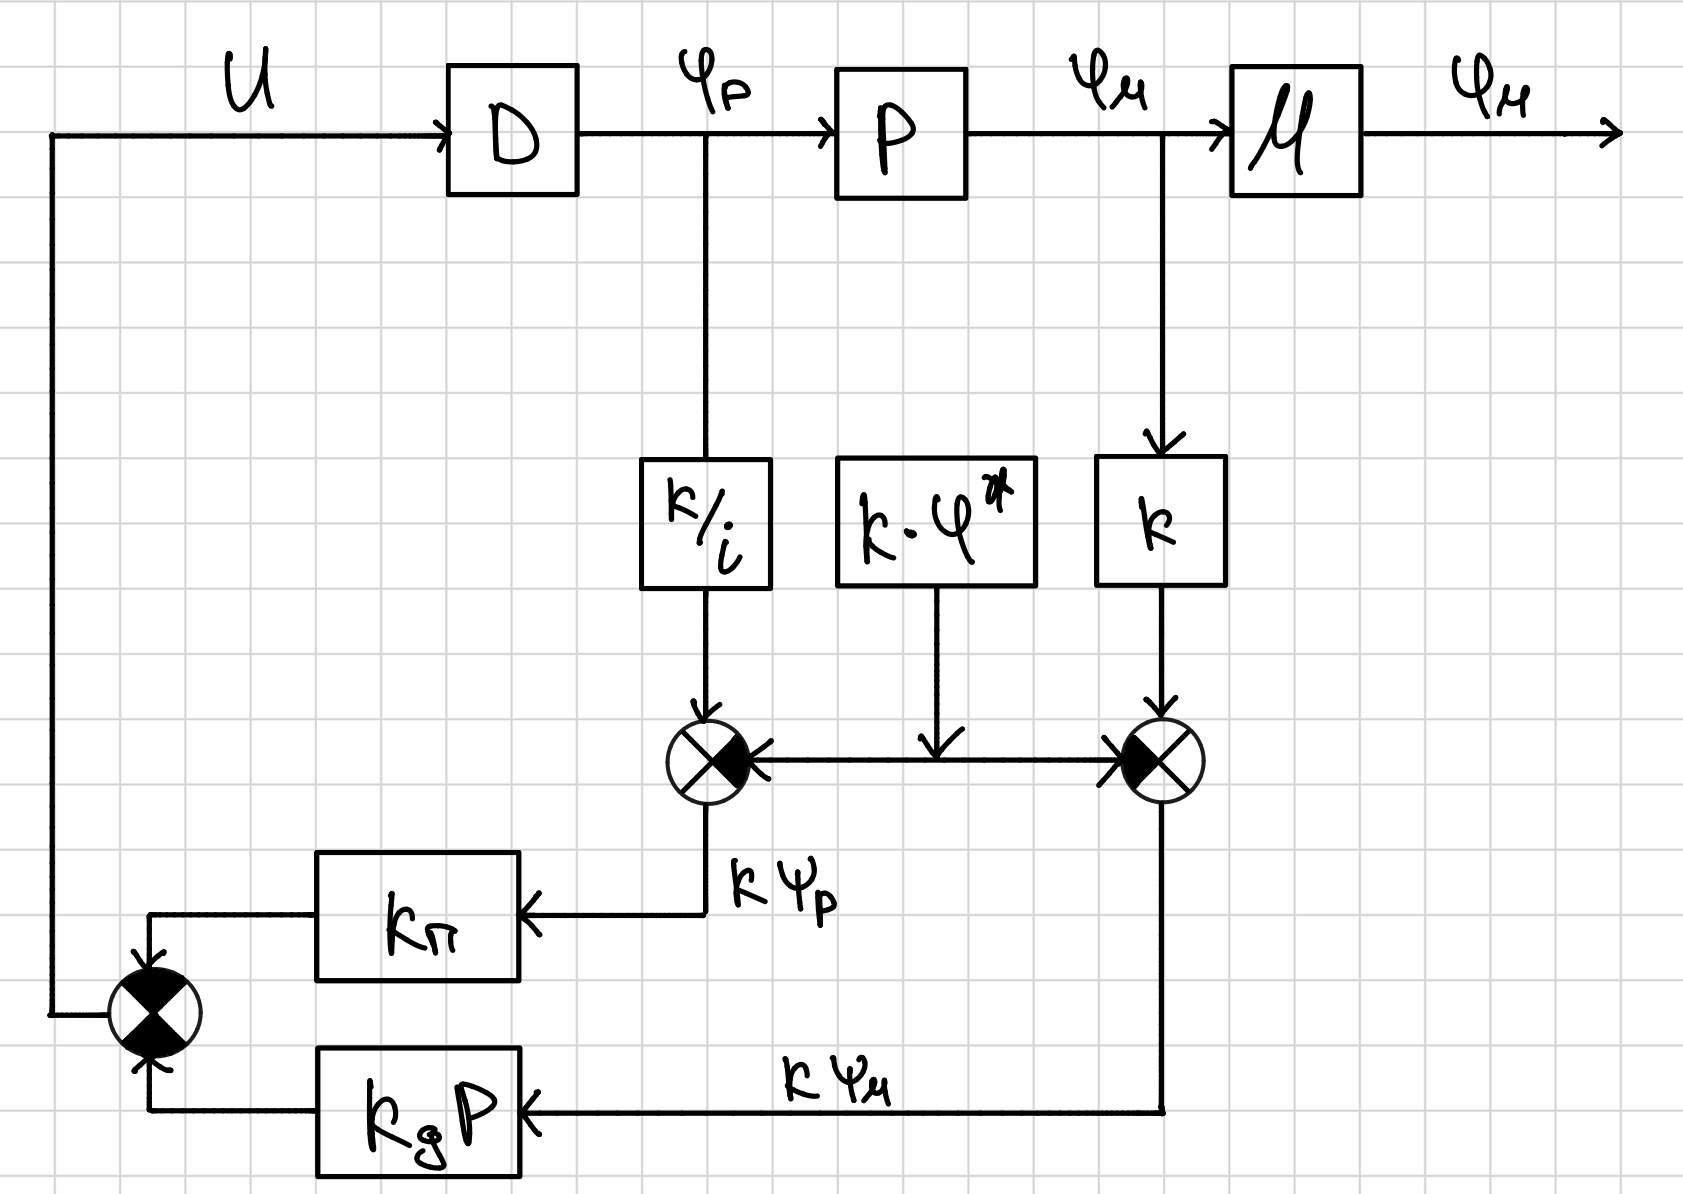
\includegraphics[width=0.75\textwidth]{graphs/fig1_drim.jpg}
    \caption{Структурная схема ДРИМ}
    \label{fig:drim}
\end{figure}

Для варианта №1 используются параметры:
\[
J_{\text{м}}=1~\text{кг}{\cdot}\text{м}^2,\quad
c=10^3~\text{Нм/рад},\quad
b=10^2~\text{Нм}{\cdot}\text{с/рад},\quad
J_{\text{д}}=2{\cdot}10^{-4}~\text{кг}{\cdot}\text{м}^2.
\]

При проведении расчётов используется линейная динамическая характеристика двигателя:
\[
\tau\dot{M}_{\text{д}}+M_{\text{д}}=-s\dot\varphi_{\text{р}}+ru,
\]
где
\[
s=0{,}2~\text{Нм}{\cdot}\text{с},\qquad
\tau=3{\cdot}10^{-3}~\text{с},\qquad
r=0{,}2~\text{Нм/В}.
\]

На диаграмме при $\varphi^*=\pi$ строятся области:
\[
\{M\}:\quad |M_{\text{м}}|_{\max}<150~\text{Нм},
\qquad
\{U\}:\quad |u|_{\max}<220~\text{В}.
\]

Допустимая область $\{L\} = \{M\}\cap\{U\}$ является пересечением этих областей.
В ней строятся линии равных длительностей переходных процессов; длительность
определяется как время окончательного вхождения в десятипроцентную полосу:
\[
|\psi_{\text{м}}(t)|\le 0{,}1\,\varphi^*.
\]

\newpage
\section{Математическая модель системы управления}

\subsection{Уравнения движения механической части}

Механическая часть модуля поворота состоит из ротора электродвигателя, редуктора и
выходного звена. Для жёсткой связи выполняется:
\[
\varphi_{\text{рпр}} = \varphi_{\text{м}},
\]
а с учётом передаточного отношения:
\[
\varphi_{\text{р}} = i\,\varphi_{\text{м}} = i\,\varphi_{\text{рпр}},\quad i=50.
\]

Кинетическая энергия системы:
\[
T = \tfrac{1}{2}J_{\text{д}}\dot\varphi_{\text{р}}^2
  + \tfrac{1}{2}J_{\text{м}}\dot\varphi_{\text{м}}^2.
\]
Переходя к приведённой координате $\varphi_{\text{рпр}}$:
\[
T = \tfrac{1}{2}J_{\text{д}}i^2\dot\varphi_{\text{рпр}}^2
  + \tfrac{1}{2}J_{\text{м}}\dot\varphi_{\text{м}}^2.
\]
Приведённый момент инерции двигателя:
\[
J_{\text{дпр}} = J_{\text{д}}\,i^2
= 2{\cdot}10^{-4}\cdot 50^2 = 0{,}5~\text{кг}{\cdot}\text{м}^2.
\]

Работа движущего момента:
\[
M_{\text{дпр}} = i\,M_{\text{д}}.
\]

Упругий момент на выходном валу редуктора:
\[
M_{\text{м}} = c(\varphi_{\text{рпр}}-\varphi_{\text{м}})
             + b(\dot\varphi_{\text{рпр}}-\dot\varphi_{\text{м}}).
\]

Система уравнений движения механической части:
\[
\begin{cases}
J_{\text{дпр}}\ddot\varphi_{\text{рпр}} = M_{\text{дпр}} - M_{\text{м}},\\
J_{\text{м}}\ddot\varphi_{\text{м}} = M_{\text{м}}.
\end{cases}
\]

\subsection{Характеристики двигателя}

Линейная динамическая характеристика двигателя в исходных переменных:
\[
\tau\dot{M}_{\text{д}} + M_{\text{д}} = -s\dot\varphi_{\text{р}} + ru.
\]
Переходя к приведённым переменным ($M_{\text{дпр}}=iM_{\text{д}}$,
$\dot\varphi_{\text{р}}=i\dot\varphi_{\text{рпр}}$):
\[
\tau\dot{M}_{\text{дпр}} + M_{\text{дпр}}
= -s\,i^2\,\dot\varphi_{\text{рпр}} + r\,i\,u.
\]
Обозначим приведённые коэффициенты:
\[
s_{\text{пр}} = s\,i^2 = 0{,}2\cdot50^2 = 500~\text{Нм}{\cdot}\text{с},
\qquad
r_{\text{пр}} = r\,i = 0{,}2\cdot50 = 10~\text{Нм/В}.
\]
Тогда:
\[
\tau\dot{M}_{\text{дпр}} + M_{\text{дпр}}
= -s_{\text{пр}}\dot\varphi_{\text{рпр}} + r_{\text{пр}}\,u.
\]

\subsection{Передаточная функция цепи обратной связи}

Структурная схема механизма с обратной связью приведена на рисунке~\ref{fig:feedback}.

\begin{figure}[H]
    \centering
    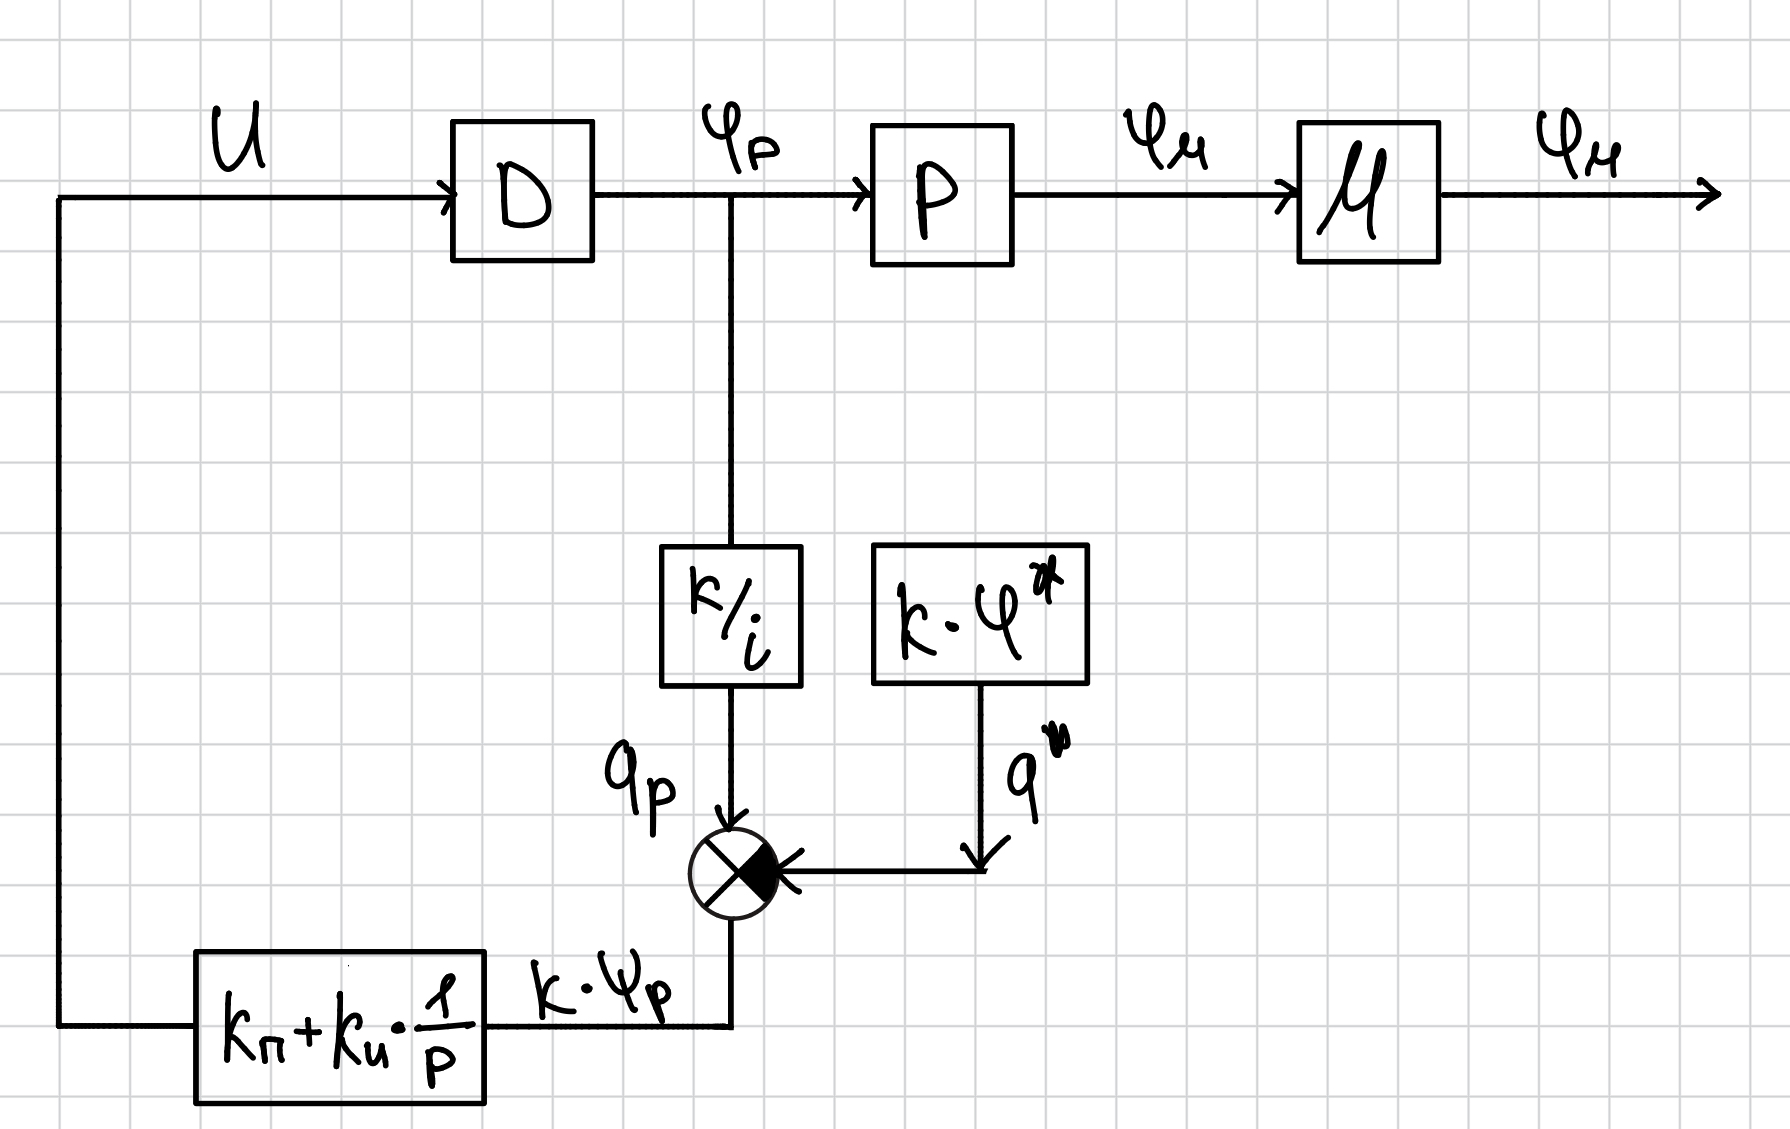
\includegraphics[width=0.75\textwidth]{graphs/fig2_feedback.jpg}
    \caption{Структурная схема механизма с обратной связью}
    \label{fig:feedback}
\end{figure}

Ошибка регулирования по приведённой координате ротора:
\[
\psi_{\text{р}} = \varphi_{\text{рпр}} - \varphi^*.
\]
Управляющее воздействие формируется ПИ-регулятором по $\psi_{\text{р}}$:
\[
u = -k\!\left(k_{\text{пр}} + \frac{k_{\text{ир}}}{p}\right)\!\psi_{\text{р}},
\]
где $k=100$~В/рад. Умножив на $p$:
\[
p\,U = -k(k_{\text{пр}}\,p + k_{\text{ир}})\,\Psi_{\text{р}}
      = -k(k_{\text{пр}}\,p + k_{\text{ир}})(\Phi_{\text{рпр}} - \Phi^*).
\]

\subsection{Операторная форма системы уравнений}

В операторной форме (Лаплас, вектор $X = [\Phi_{\text{рпр}},\,\Phi_{\text{м}},\,\overline{M}_{\text{дпр}},\,U]^T$):
\[
\begin{cases}
(J_{\text{дпр}}p^2+bp+c)\,\Phi_{\text{рпр}} - (bp+c)\,\Phi_{\text{м}} - \overline{M}_{\text{дпр}} = 0,\\
-(bp+c)\,\Phi_{\text{рпр}} + (J_{\text{м}}p^2+bp+c)\,\Phi_{\text{м}} = 0,\\
s_{\text{пр}}\,p\,\Phi_{\text{рпр}} + (\tau p+1)\,\overline{M}_{\text{дпр}} - r_{\text{пр}}\,U = 0,\\
k(k_{\text{пр}}\,p+k_{\text{ир}})\,\Phi_{\text{рпр}} + p\,U
= k(k_{\text{пр}}\,p+k_{\text{ир}})\,\Phi^*.
\end{cases}
\]

\subsection{Матричная форма системы}

Систему запишем в виде $AX = h\Phi^*$, где:
\[
A=
\begin{bmatrix}
J_{\text{дпр}}p^2+bp+c & -(bp+c) & -1 & 0\\
-(bp+c) & J_{\text{м}}p^2+bp+c & 0 & 0\\
s_{\text{пр}}\,p & 0 & \tau p+1 & -r_{\text{пр}}\\
k(k_{\text{пр}}p+k_{\text{ир}}) & 0 & 0 & p
\end{bmatrix},
\quad
h=
\begin{bmatrix}0\\0\\0\\k(k_{\text{пр}}p+k_{\text{ир}})\end{bmatrix}.
\]

После подстановки числовых значений:
\[
A=
\begin{bmatrix}
0{,}5p^2+100p+1000 & -(100p+1000) & -1 & 0\\
-(100p+1000) & p^2+100p+1000 & 0 & 0\\
500p & 0 & 0{,}003p+1 & -10\\
100(k_{\text{пр}}p+k_{\text{ир}}) & 0 & 0 & p
\end{bmatrix}.
\]

\subsection{Структурная схема системы управления}

Из операторной формы системы выразим каждую переменную через входные воздействия.
Механическая часть:
\[
\begin{cases}
\Phi_{\text{рпр}}=\dfrac{\overline{M}_{\text{дпр}}+(bp+c)\,\Phi_{\text{м}}}
{J_{\text{дпр}}p^2+bp+c},\\[8pt]
\Phi_{\text{м}}=\dfrac{(bp+c)\,\Phi_{\text{рпр}}}{J_{\text{м}}p^2+bp+c}.
\end{cases}
\]
Двигатель:
\[
\overline{M}_{\text{дпр}}=\frac{r_{\text{пр}}\,U - s_{\text{пр}}\,p\,\Phi_{\text{рпр}}}{\tau p+1}.
\]
Закон управления (ПИ-регулятор по ротору):
\[
U = -k\!\left(k_{\text{пр}}+\frac{k_{\text{ир}}}{p}\right)(\Phi_{\text{рпр}}-\Phi^*).
\]

Структурная схема системы управления приведена на рисунке~\ref{fig:block_scheme}.

\begin{figure}[H]
    \centering
    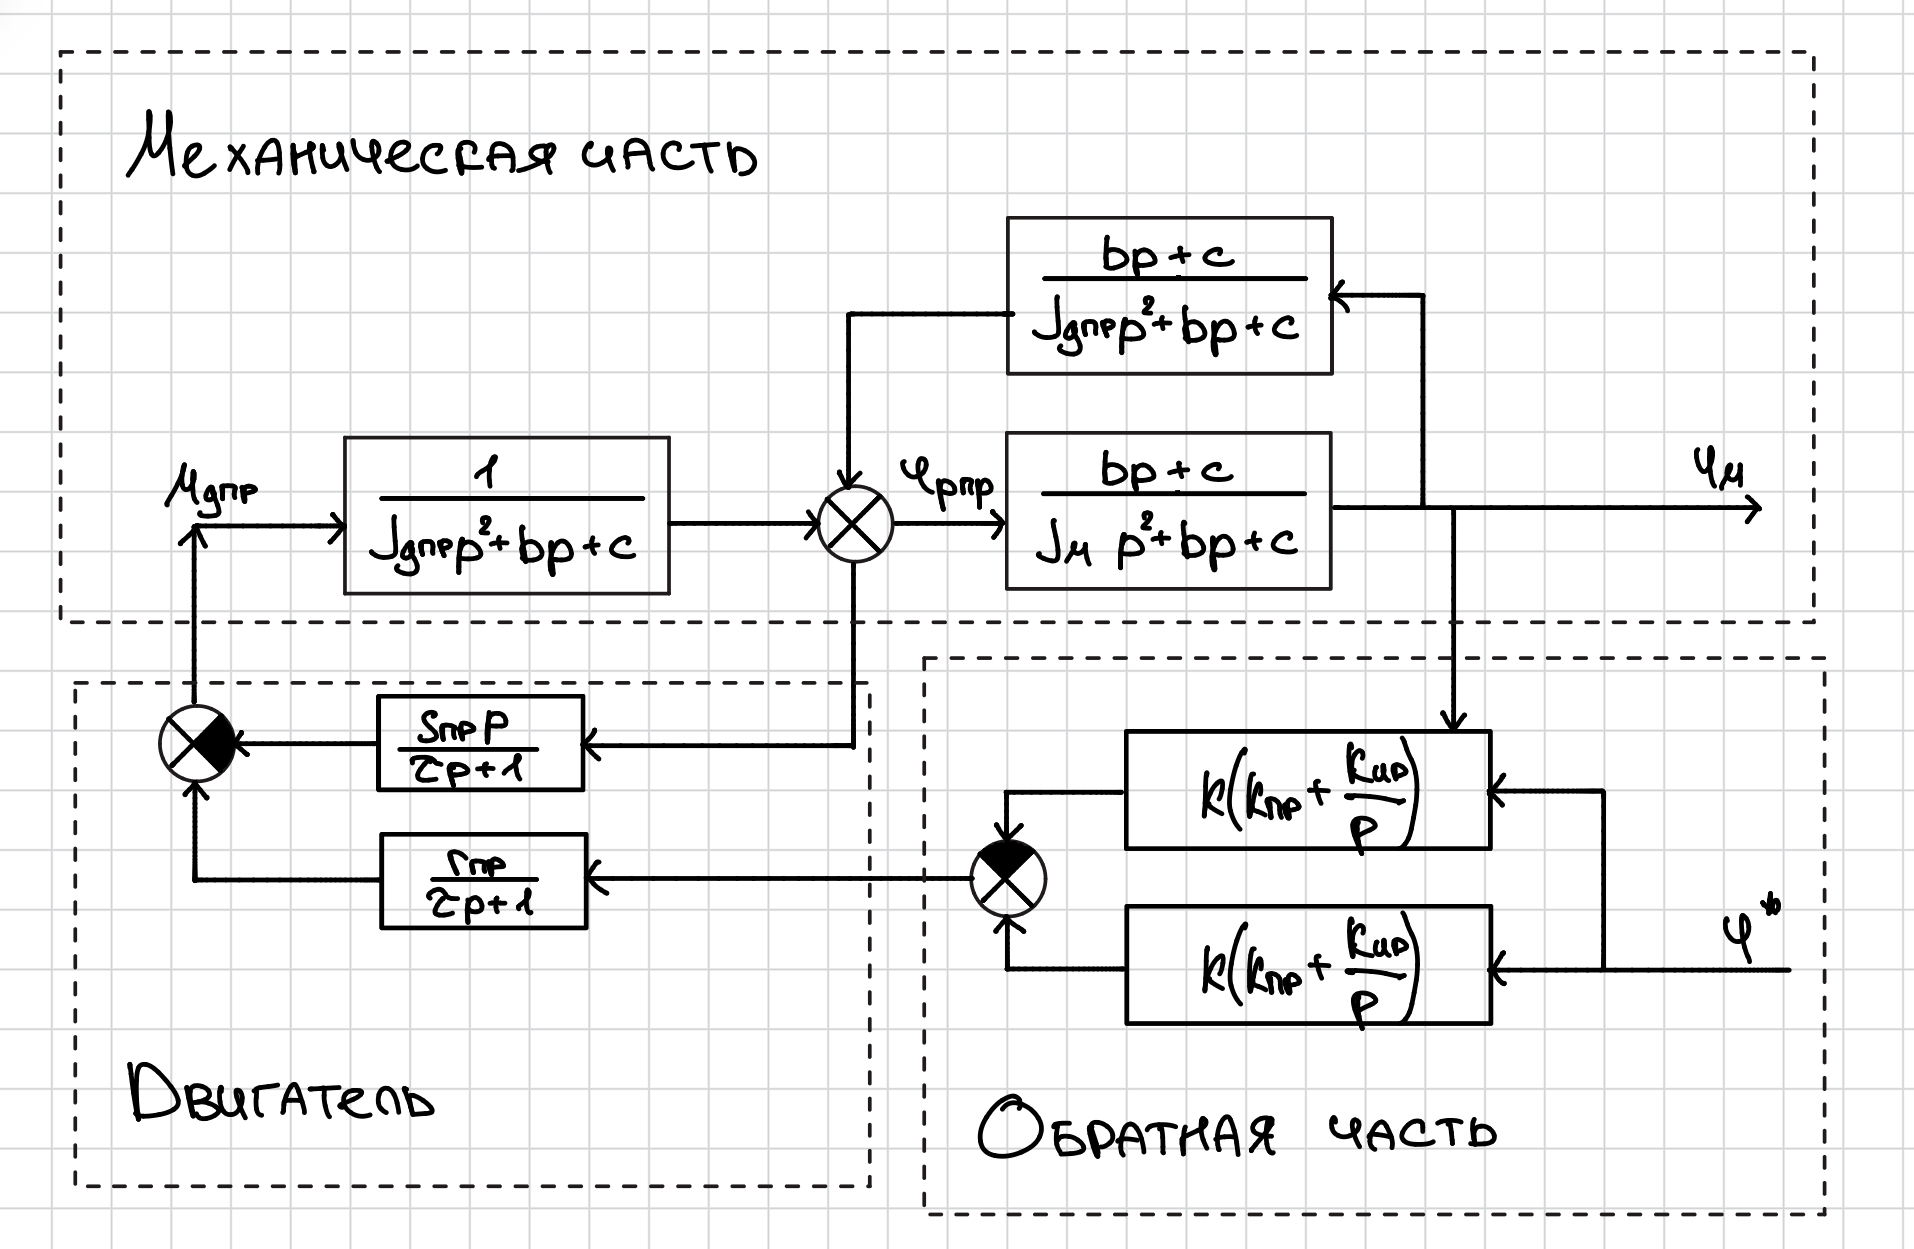
\includegraphics[width=0.95\textwidth]{graphs/fig3_block_scheme.jpg}
    \caption{Структурная схема системы управления}
    \label{fig:block_scheme}
\end{figure}

\newpage
\section[Область устойчивости в пространстве параметров]
        {Область устойчивости в пространстве параметров $(k_{\text{пр}},\,k_{\text{ир}})$}

\subsection{Характеристическое уравнение}

Знаменатель передаточных функций определяется как $D(p)=\det A$. Вычисляя
определитель и раскрывая скобки, получим характеристическое уравнение шестой
степени:
\[
D(p) =
\frac{3}{2000}p^6
+\frac{19}{20}p^5
+\frac{1309}{2}p^4
+(1000k_{\text{пр}}+51500)\,p^3
\]
\[
+(1000k_{\text{ир}}+100000k_{\text{пр}}+500000)\,p^2
+(100000k_{\text{ир}}+1000000k_{\text{пр}})\,p
+1000000k_{\text{ир}} = 0.
\]

Обозначим коэффициенты:
\[
a_6=\frac{3}{2000}=0{,}0015,\quad
a_5=\frac{19}{20}=0{,}95,\quad
a_4=\frac{1309}{2}=654{,}5,
\]
\[
a_3=1000k_{\text{пр}}+51500,\quad
a_2=1000k_{\text{ир}}+100000k_{\text{пр}}+500000,
\]
\[
a_1=100000k_{\text{ир}}+1000000k_{\text{пр}},\quad
a_0=1000000k_{\text{ир}}.
\]

\subsection{Критерий Стодолы и Рауса--Гурвица}

По критерию Стодолы необходимое условие устойчивости --- положительность всех
коэффициентов характеристического уравнения $a_i>0$. Поскольку $a_6,\,a_5,\,a_4>0$
всегда, получаем:
\[
k_{\text{ир}}>0,
\]
\[
k_{\text{пр}}>-51{,}5\quad\text{(при }k_{\text{пр}}\ge0\text{ выполняется автоматически)},
\]
\[
100\,k_{\text{пр}}+k_{\text{ир}}>-500\quad\text{(выполняется при }k_{\text{пр}},k_{\text{ир}}>0\text{)},
\]
\[
0{,}1\,k_{\text{ир}}+k_{\text{пр}}>0\quad\text{(выполняется при }k_{\text{пр}},k_{\text{ир}}>0\text{)}.
\]

Для полинома шестой степени матрица Гурвица $5\times5$ строится по стандартной
схеме. Элементы таблицы Рауса:
\[
b_1 = \frac{a_5 a_4 - a_6 a_3}{a_5}
= 654{,}5 - \frac{3}{1900}(1000k_{\text{пр}}+51500)
= 573{,}25 - \frac{3k_{\text{пр}}}{1{,}9}.
\]
Условие $b_1>0$ выполняется при $k_{\text{пр}}<363$, что заведомо справедливо в
исследуемом диапазоне.

Условия на $c_1>0$, $d_1>0$ и $e_1>0$ (определители Гурвица старших порядков)
являются нелинейными функциями параметров и вычисляются численно. На их основе
строится граница области устойчивости в плоскости $(k_{\text{пр}},\,k_{\text{ир}})$.

Полученная область устойчивости показана на рисунке~\ref{fig:stability}.

\begin{figure}[H]
    \centering
    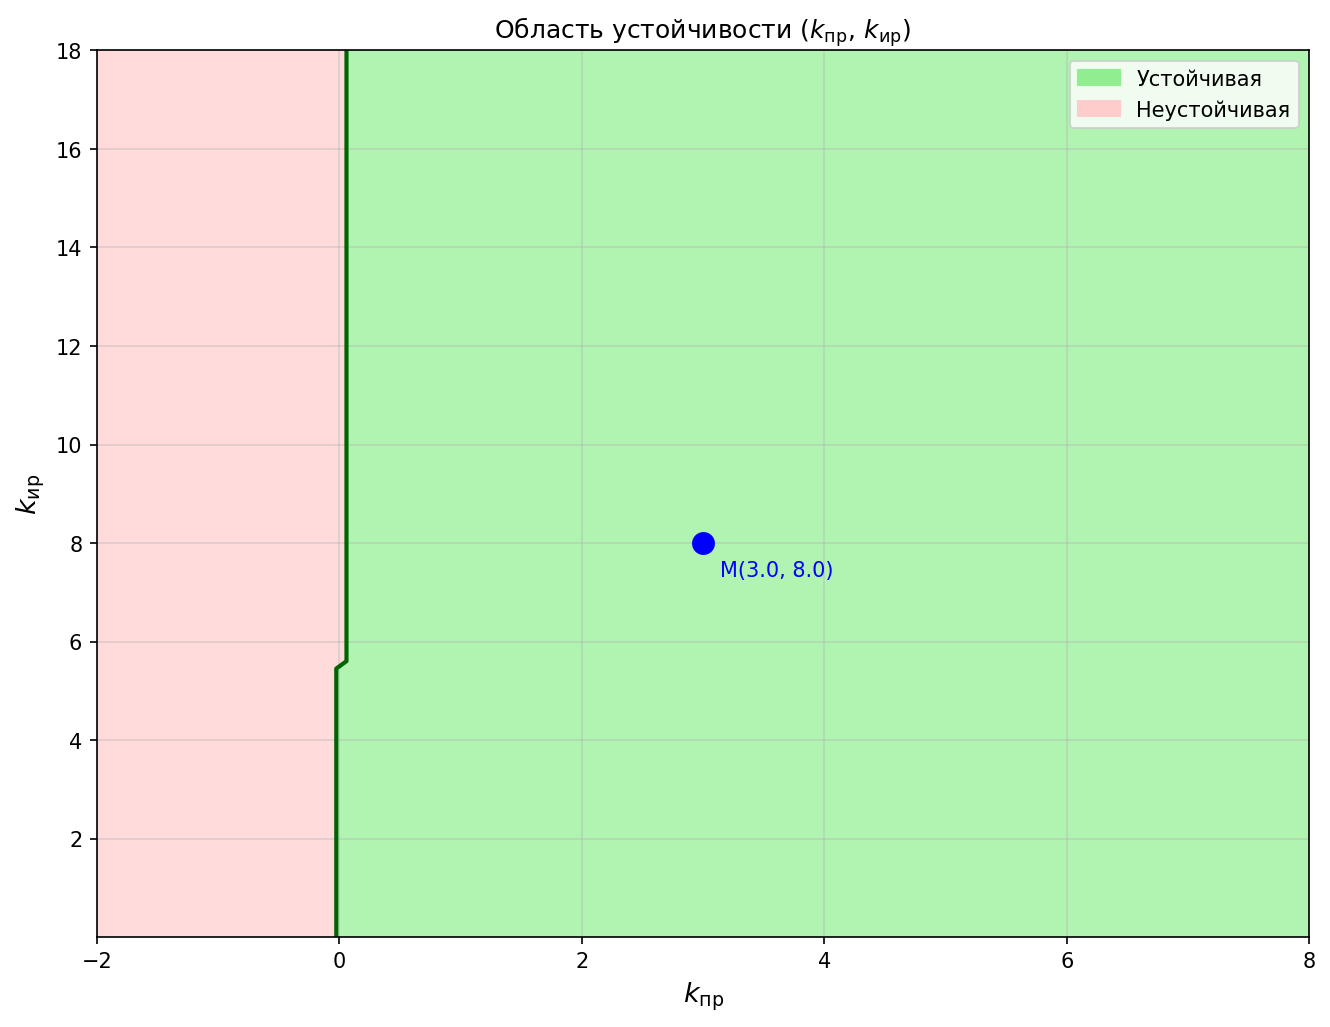
\includegraphics[width=0.9\textwidth]{graphs/stability_region.png}
    \caption{Область устойчивости замкнутой системы управления
             в пространстве параметров $(k_{\text{пр}},\,k_{\text{ир}})$}
    \label{fig:stability}
\end{figure}

Зелёная область соответствует парам $(k_{\text{пр}},\,k_{\text{ир}})$, при которых
все условия Рауса--Гурвица выполнены и замкнутая система устойчива. Красноватая
область~--- точки, не удовлетворяющие хотя бы одному условию устойчивости.
Синяя точка $M(3;\,8)$ выбрана внутри зелёной области для проверки по критерию
Михайлова.

\subsection{Проверка устойчивости по годографу Михайлова}

Для проверки выберем точку $M$ внутри области устойчивости:
\[
k_{\text{пр}} = 3{,}0,\qquad k_{\text{ир}} = 8{,}0.
\]
Для этой точки характеристический полином принимает вид:
\[
D(p) = 0{,}0015p^6 + 0{,}95p^5 + 654{,}5p^4
+ 54500\,p^3 + 1308000\,p^2 + 3800000\,p + 8000000.
\]

Полагая $p=j\omega$, годограф Михайлова $D(j\omega)=P(\omega)+jQ(\omega)$:
\[
P(\omega) = 0{,}0015\omega^6 - 654{,}5\omega^4 + 1308000\,\omega^2 - 8000000,
\]
\[
Q(\omega) = -0{,}95\omega^5 + 54500\,\omega^3 + 3800000\,\omega.
\]
(Знаки соответствуют подстановке $j^n$: $j^6=-1$, $j^5=-j$ и т.д.)

При $\omega=0$:
\[
D(0) = a_0 = 10^6\cdot k_{\text{ир}} = 8\cdot10^6 > 0.
\]
Так как степень полинома равна шести, для устойчивой системы годограф Михайлова
при изменении $\omega$ от $0$ до $+\infty$ должен пройти шесть квадрантов,
повернувшись на угол $3\pi$.

Корни характеристического полинома в точке $M$:
\[
p_{1,2} = -270{,}46 \pm 558{,}40j,\quad
p_{3,4} = -3{,}03 \pm 2{,}67j,
\]
\[
p_5 = -75{,}02,\quad
p_6 = -11{,}33.
\]
Все корни имеют отрицательные вещественные части, что подтверждает устойчивость.

\begin{figure}[H]
    \centering
    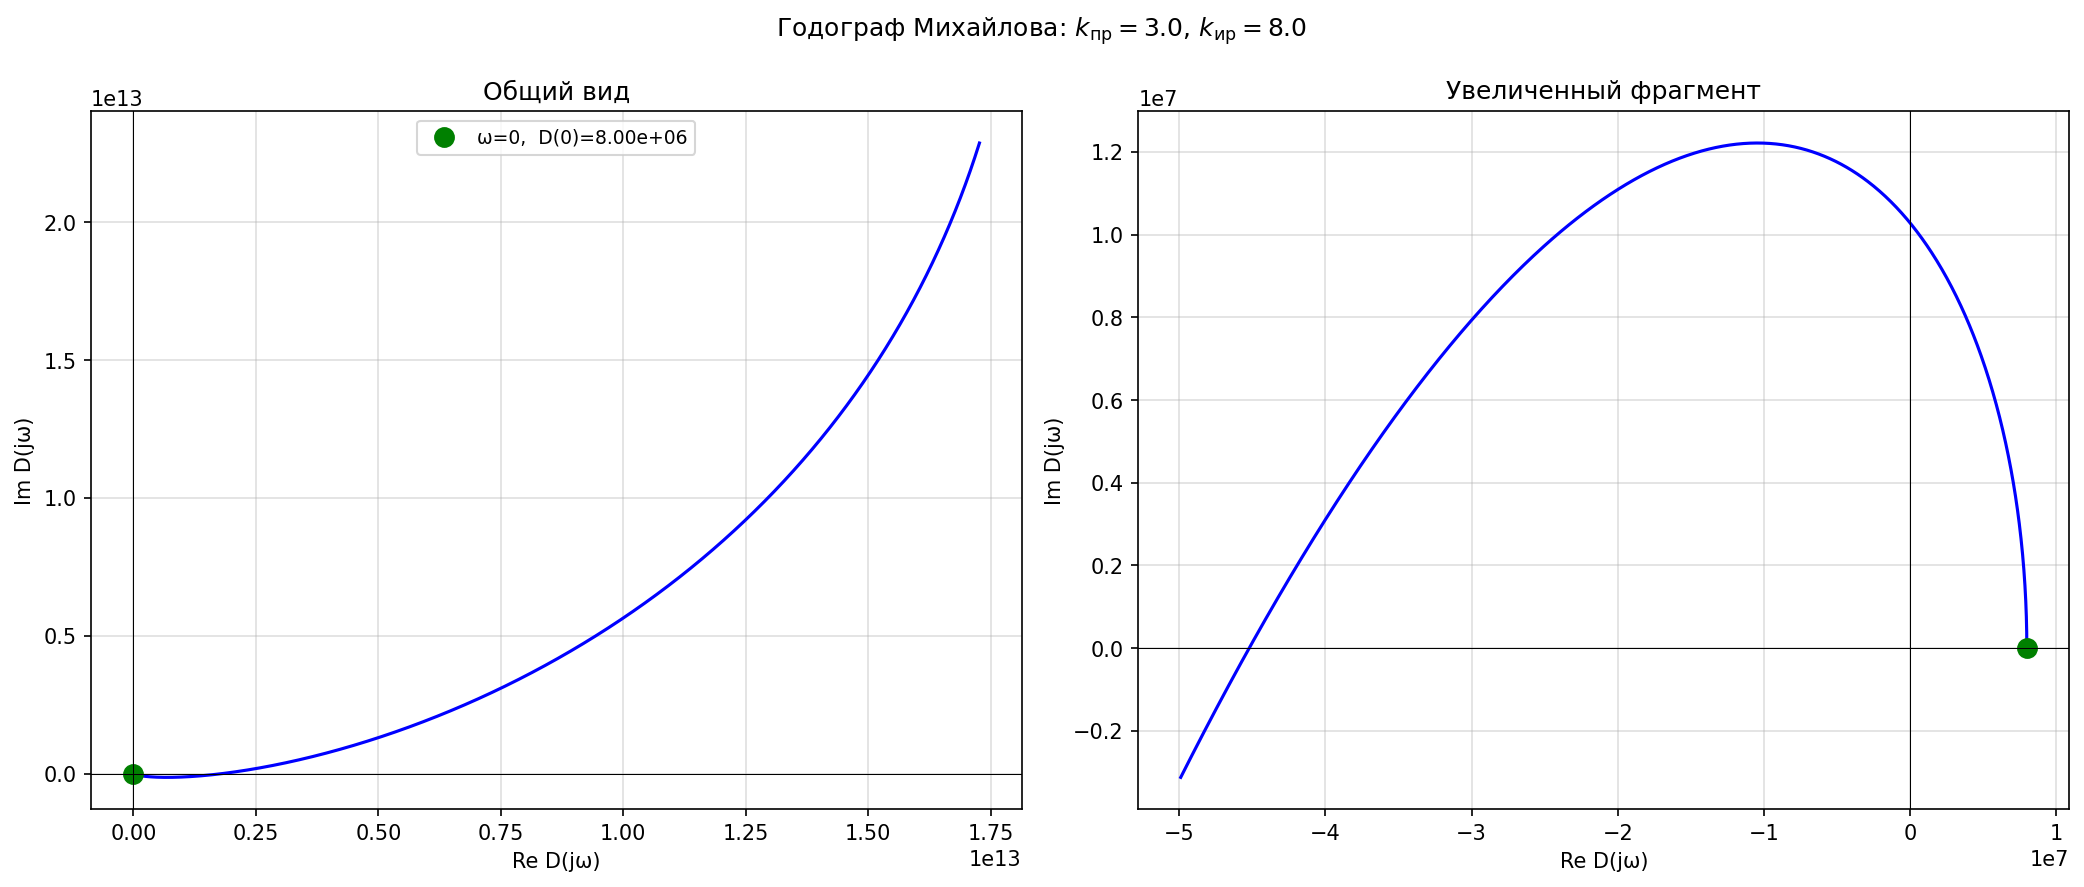
\includegraphics[width=0.9\textwidth]{graphs/mikhailov.png}
    \caption{Годограф Михайлова для точки $k_{\text{пр}}=3{,}0$, $k_{\text{ир}}=8{,}0$}
    \label{fig:mikhailov}
\end{figure}

Годограф начинается на положительной вещественной оси ($D(0)=8\cdot10^6$) и
при увеличении $\omega$ последовательно проходит требуемое число квадрантов.
Следовательно, по критерию Михайлова выбранная точка принадлежит области
устойчивости.

\newpage
\section{Исследование переходных процессов}

\subsection{Система дифференциальных уравнений в переменных состояния}

Введём вектор состояния:
\[
x = \begin{bmatrix}x_1&x_2&x_3&x_4&x_5&x_6\end{bmatrix}^T
  = \begin{bmatrix}
    \varphi_{\text{рпр}}&
    \dot\varphi_{\text{рпр}}&
    \varphi_{\text{м}}&
    \dot\varphi_{\text{м}}&
    M_{\text{дпр}}&
    \xi
    \end{bmatrix}^T,
\]
где $\xi = \int_0^t\psi_{\text{р}}\,d\tau'$ --- интеграл ошибки по ротору.

Закон управления:
\[
u = -k\bigl(k_{\text{пр}}\psi_{\text{р}} + k_{\text{ир}}\,\xi\bigr)
  = -100\bigl(k_{\text{пр}}(x_1-\pi) + k_{\text{ир}}\,x_6\bigr).
\]

Система уравнений движения:
\[
\begin{cases}
\dot x_1 = x_2,\\[4pt]
\dot x_2 = \dfrac{x_5 - b(x_2-x_4) - c(x_1-x_3)}{J_{\text{дпр}}}
         = 2\bigl[x_5 - 100(x_2-x_4) - 1000(x_1-x_3)\bigr],\\[4pt]
\dot x_3 = x_4,\\[4pt]
\dot x_4 = \dfrac{b(x_2-x_4)+c(x_1-x_3)}{J_{\text{м}}}
         = 100(x_2-x_4)+1000(x_1-x_3),\\[4pt]
\dot x_5 = \dfrac{-x_5 - s_{\text{пр}}\,x_2 + r_{\text{пр}}\,u}{\tau}
         = \dfrac{-x_5 - 500\,x_2 + 10\,u}{0{,}003},\\[4pt]
\dot x_6 = x_1 - \pi.
\end{cases}
\]
Начальные условия нулевые: $x(0)=\mathbf{0}$.

Начальное значение управляющего сигнала:
\[
u(0) = -100\,k_{\text{пр}}\,(0-\pi) = 100\pi\,k_{\text{пр}}.
\]
Чтобы уже в момент $t=0$ не превысить $220$~В, необходимо:
\[
100\pi\,k_{\text{пр}} < 220
\quad\Rightarrow\quad
k_{\text{пр}} < \frac{220}{100\pi} \approx 0{,}700.
\]

По рассчитанным состояниям определяются:
\[
M_{\text{м}} = c(x_1-x_3)+b(x_2-x_4)
= 1000(x_1-x_3)+100(x_2-x_4),
\]
\[
u = -100\bigl(k_{\text{пр}}(x_1-\pi)+k_{\text{ир}}\,x_6\bigr).
\]
Численное интегрирование выполнялось методом LSODA (адаптивный порядок). Для
переходных процессов шаг задавался адаптивно с $\varepsilon_{\text{rel}}=10^{-6}$.

\subsection{Характерные переходные процессы}

Рассмотрим три характерные точки области устойчивости.

\textbf{Точка 1}: $k_{\text{пр}}=0{,}20$, $k_{\text{ир}}=0{,}50$ --- типичная
внутренняя точка. Начальное напряжение:
\[
u(0) = 100\pi\cdot0{,}20 = 62{,}83~\text{В}.
\]
Переходный процесс показан на рисунке~\ref{fig:trans_inside}. Оба ограничения
выполняются с запасом.

\begin{figure}[H]
    \centering
    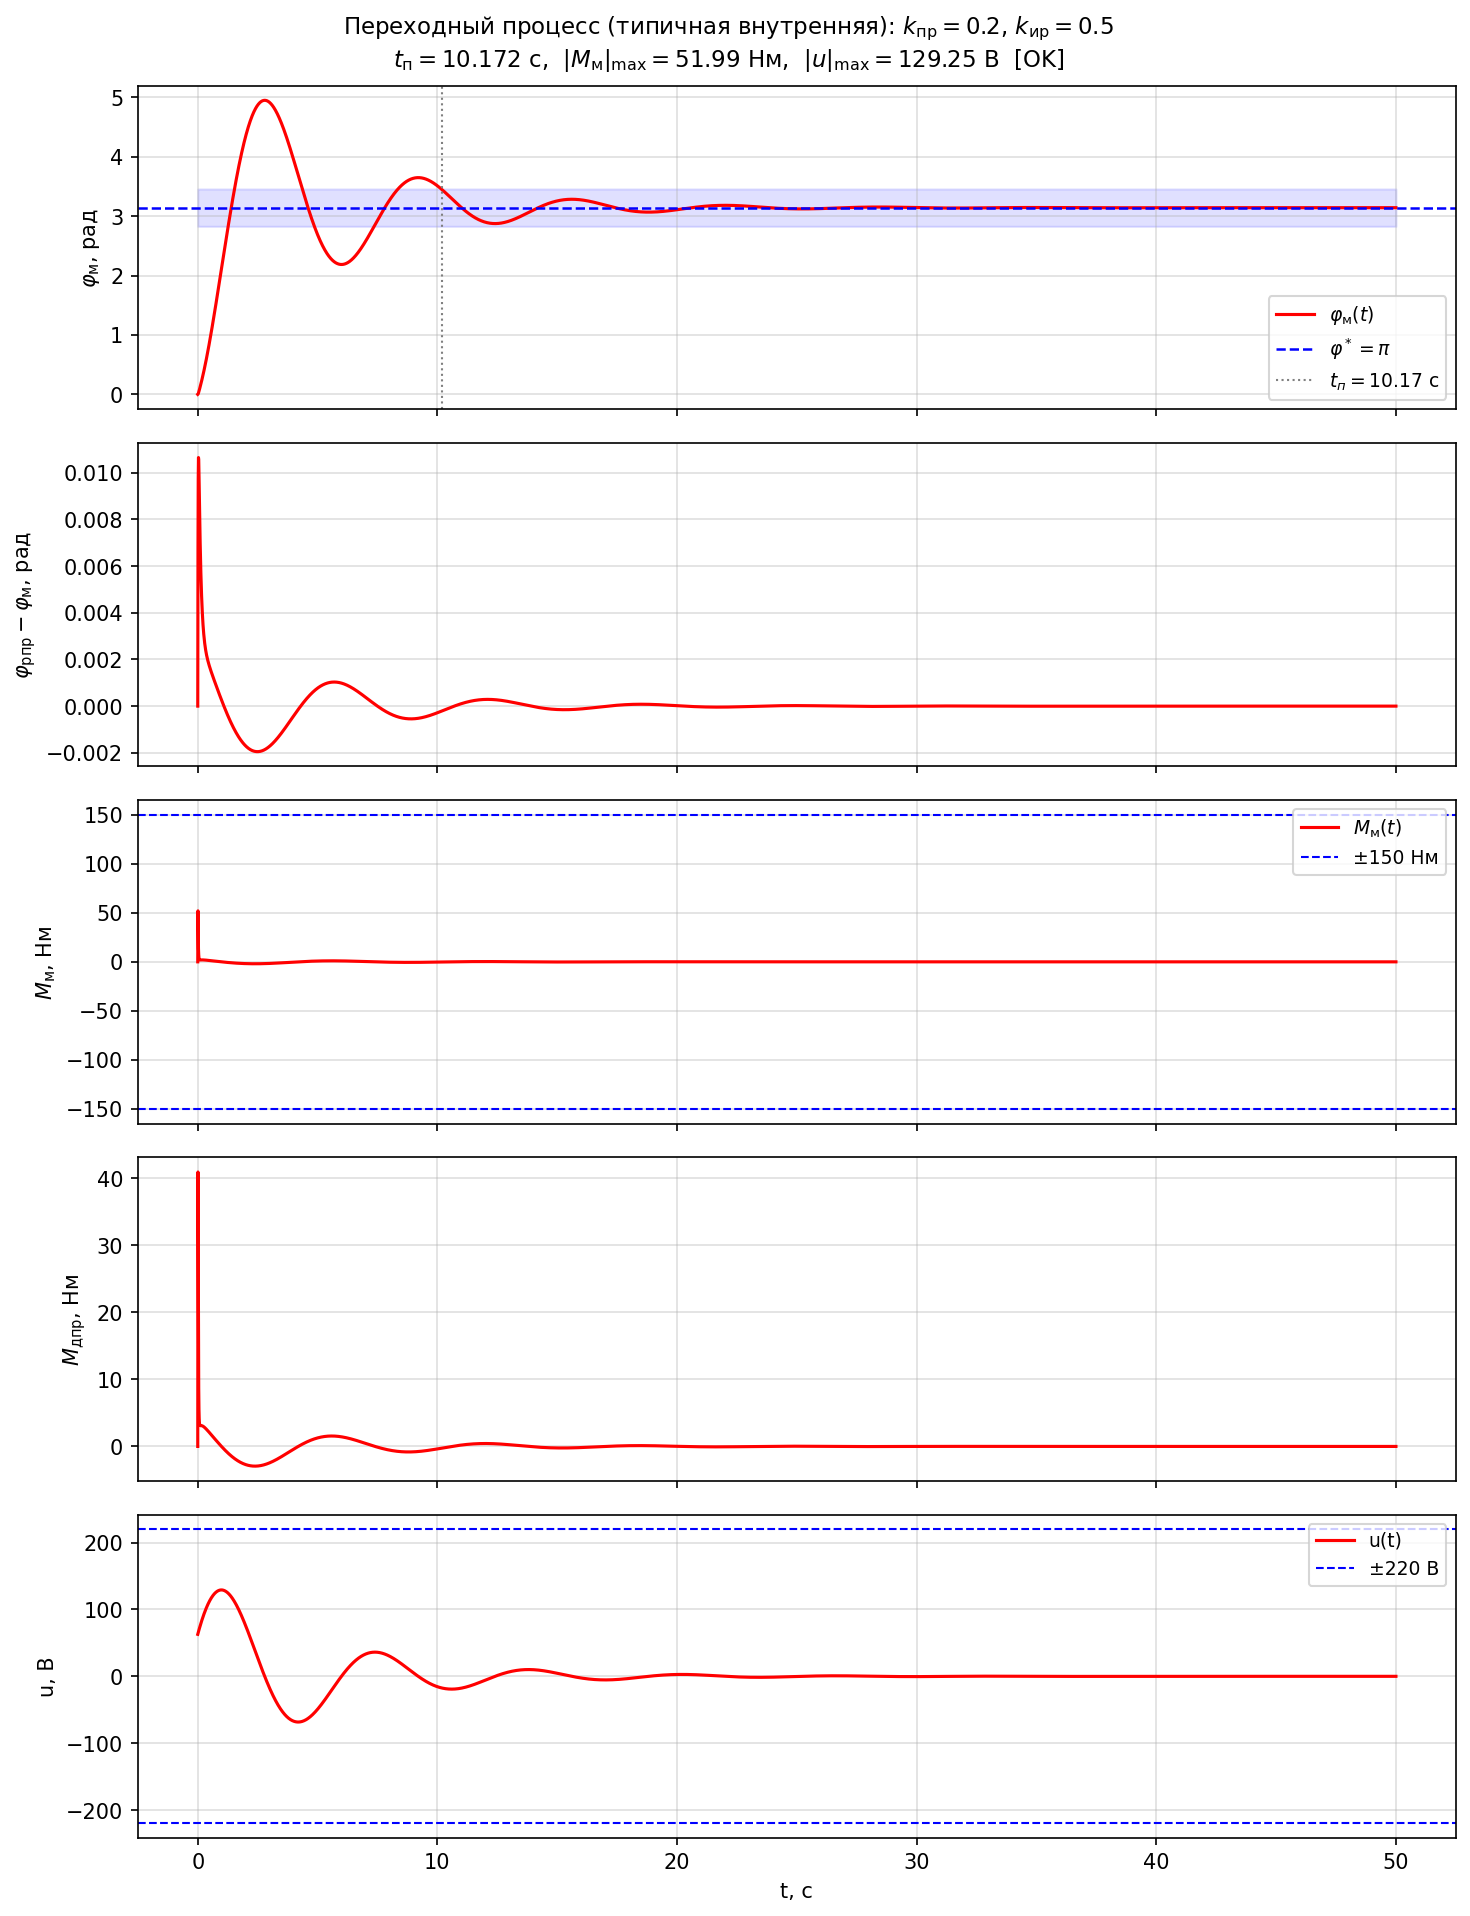
\includegraphics[width=0.95\textwidth]{graphs/transient_inside.png}
    \caption{Переходный процесс при $k_{\text{пр}}=0{,}20$, $k_{\text{ир}}=0{,}50$}
    \label{fig:trans_inside}
\end{figure}

\textbf{Точка 2}: $k_{\text{пр}}=0{,}05$, $k_{\text{ир}}=0{,}80$ --- малый
пропорциональный коэффициент, относительно большой интегральный. Начальное напряжение
$u(0)=15{,}71$~В. Момент мал ($M_{\text{м}}\ll 150$~Нм), но переходный процесс
значительно затягивается.

\begin{figure}[H]
    \centering
    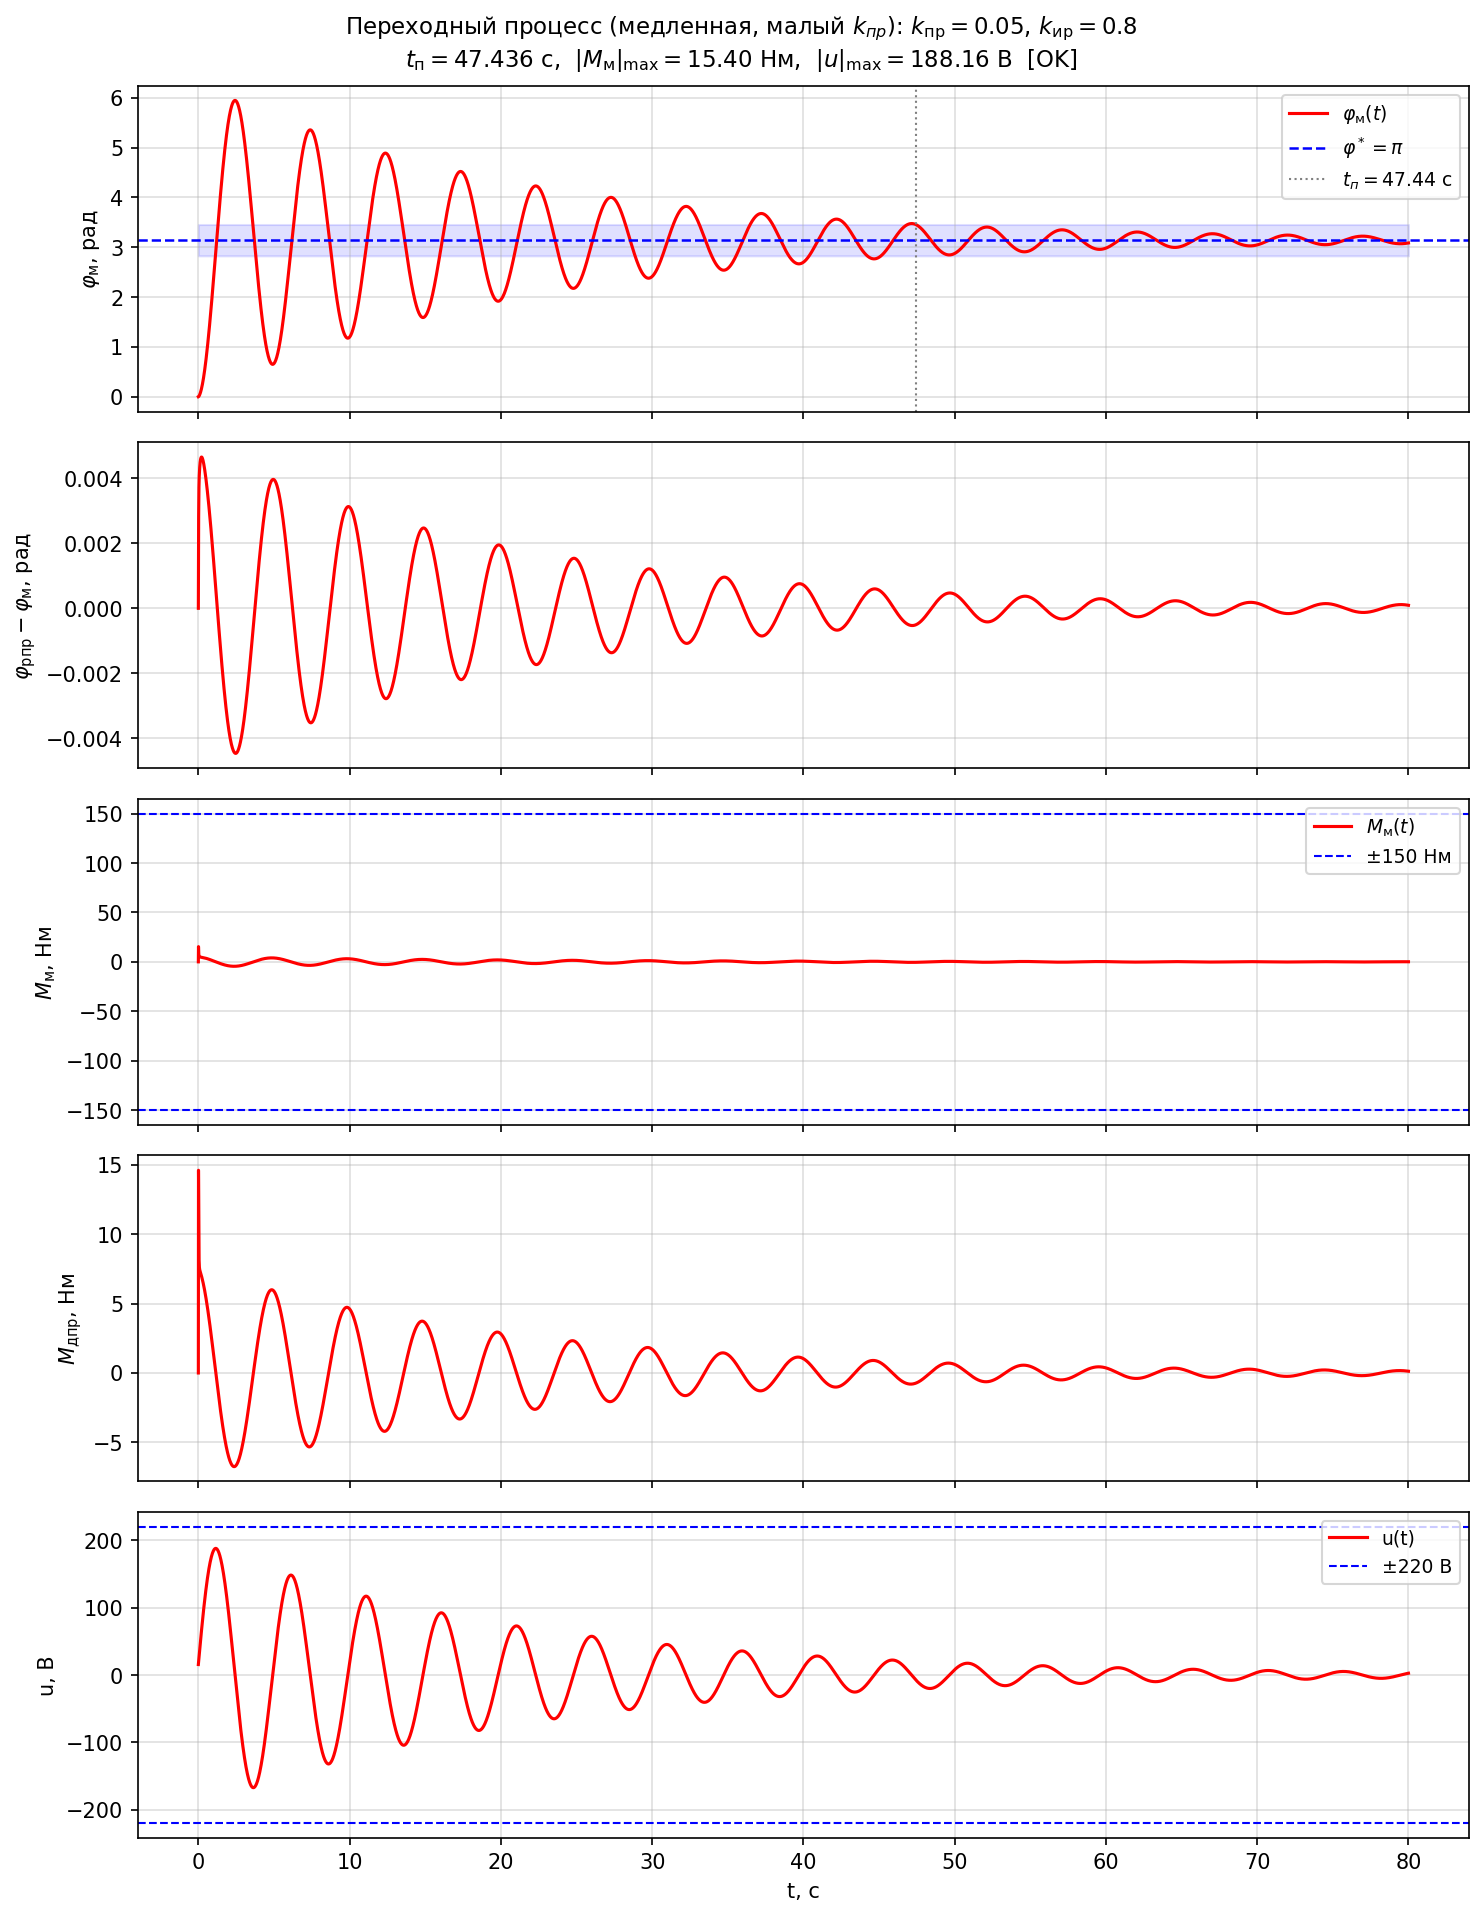
\includegraphics[width=0.95\textwidth]{graphs/transient_slow.png}
    \caption{Переходный процесс при $k_{\text{пр}}=0{,}05$, $k_{\text{ир}}=0{,}80$
             (вблизи нижней границы по $k_{\text{пр}}$)}
    \label{fig:trans_slow}
\end{figure}

\textbf{Итог по двум точкам}: увеличение $k_{\text{пр}}$ при постоянном
$k_{\text{ир}}$ ускоряет переходный процесс и увеличивает крутящий момент;
увеличение $k_{\text{ир}}$ улучшает точность по интегралу ошибки, но повышает
максимальное управляющее напряжение. Наиболее жёстким из двух ограничений для
данного варианта является ограничение по управляющему сигналу при больших $k_{\text{ир}}$
и ограничение по моменту при больших $k_{\text{пр}}$.

\subsection{Область допустимых значений крутящего момента}

Для каждой устойчивой точки сетки
$k_{\text{пр}}\in[0{,}03;\,0{,}27]$,\; $k_{\text{ир}}\in[0{,}1;\,1{,}3]$
рассчитывался максимум:
\[
|M_{\text{м}}|_{\max} = \max_t\bigl|1000(x_1-x_3)+100(x_2-x_4)\bigr|.
\]
Область $\{M\}$, в которой $|M_{\text{м}}|_{\max}<150$~Нм, показана на
рисунке~\ref{fig:torque}.

\begin{figure}[H]
    \centering
    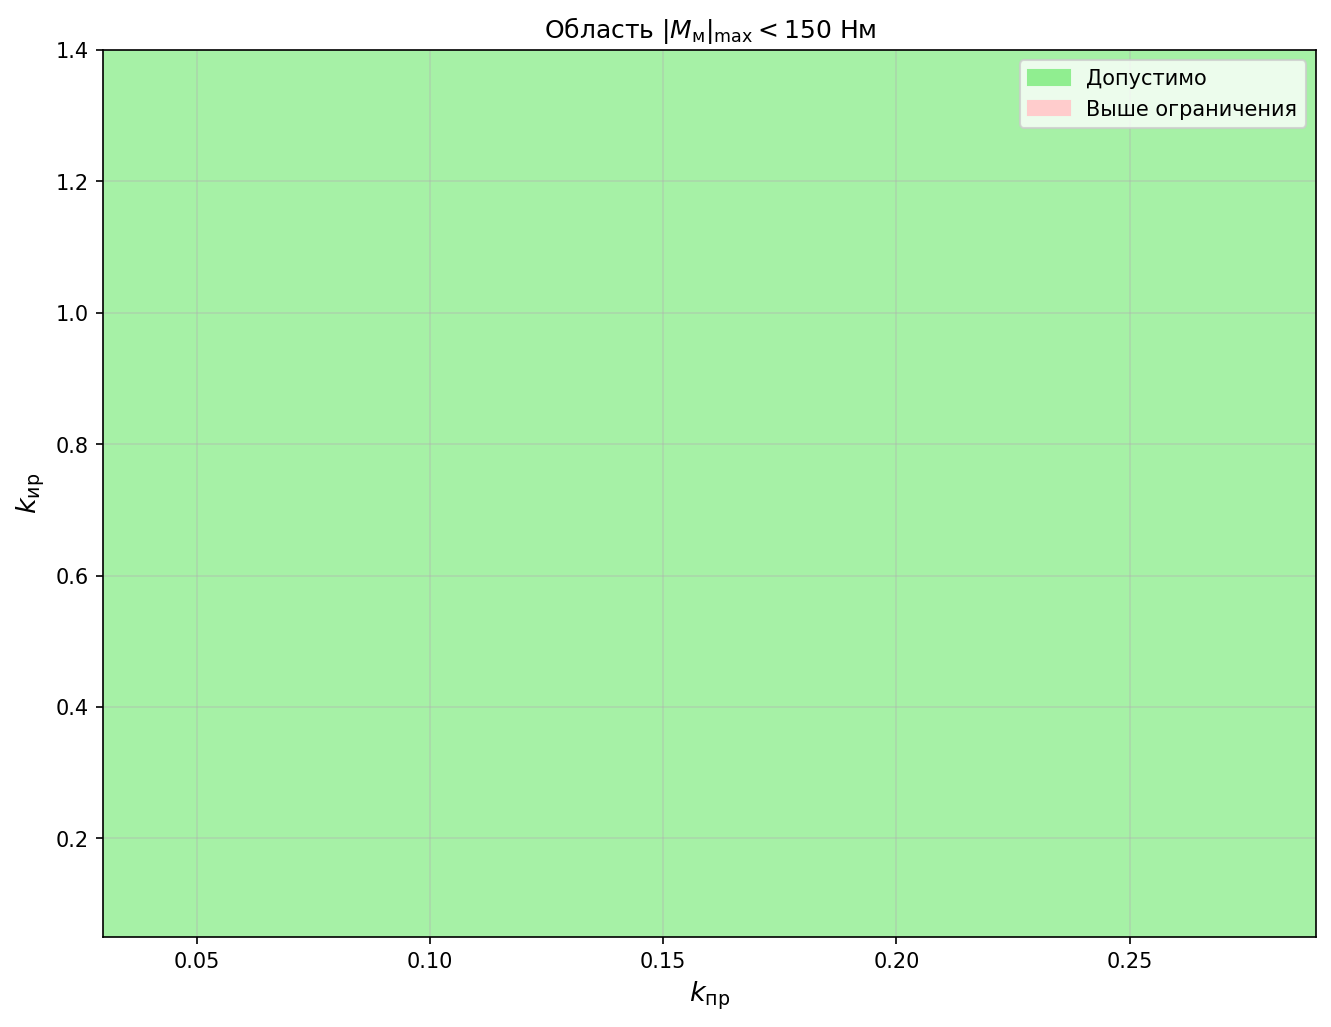
\includegraphics[width=0.9\textwidth]{graphs/torque_region.png}
    \caption{Область допустимых значений крутящего момента
             $|M_{\text{м}}|_{\max}<150$~Нм}
    \label{fig:torque}
\end{figure}

\subsection{Область допустимых значений управляющего сигнала}

Аналогично вычислялся максимум управляющего сигнала:
\[
|u|_{\max} = \max_t\bigl|{-100\bigl(k_{\text{пр}}(x_1-\pi)+k_{\text{ир}}\,x_6\bigr)}\bigr|.
\]
Поскольку $u(0)=100\pi\,k_{\text{пр}}$, граница $|u|_{\max}=220$~В в основном
определяется значением $k_{\text{пр}}$. Область $\{U\}$ показана на
рисунке~\ref{fig:voltage}.

\begin{figure}[H]
    \centering
    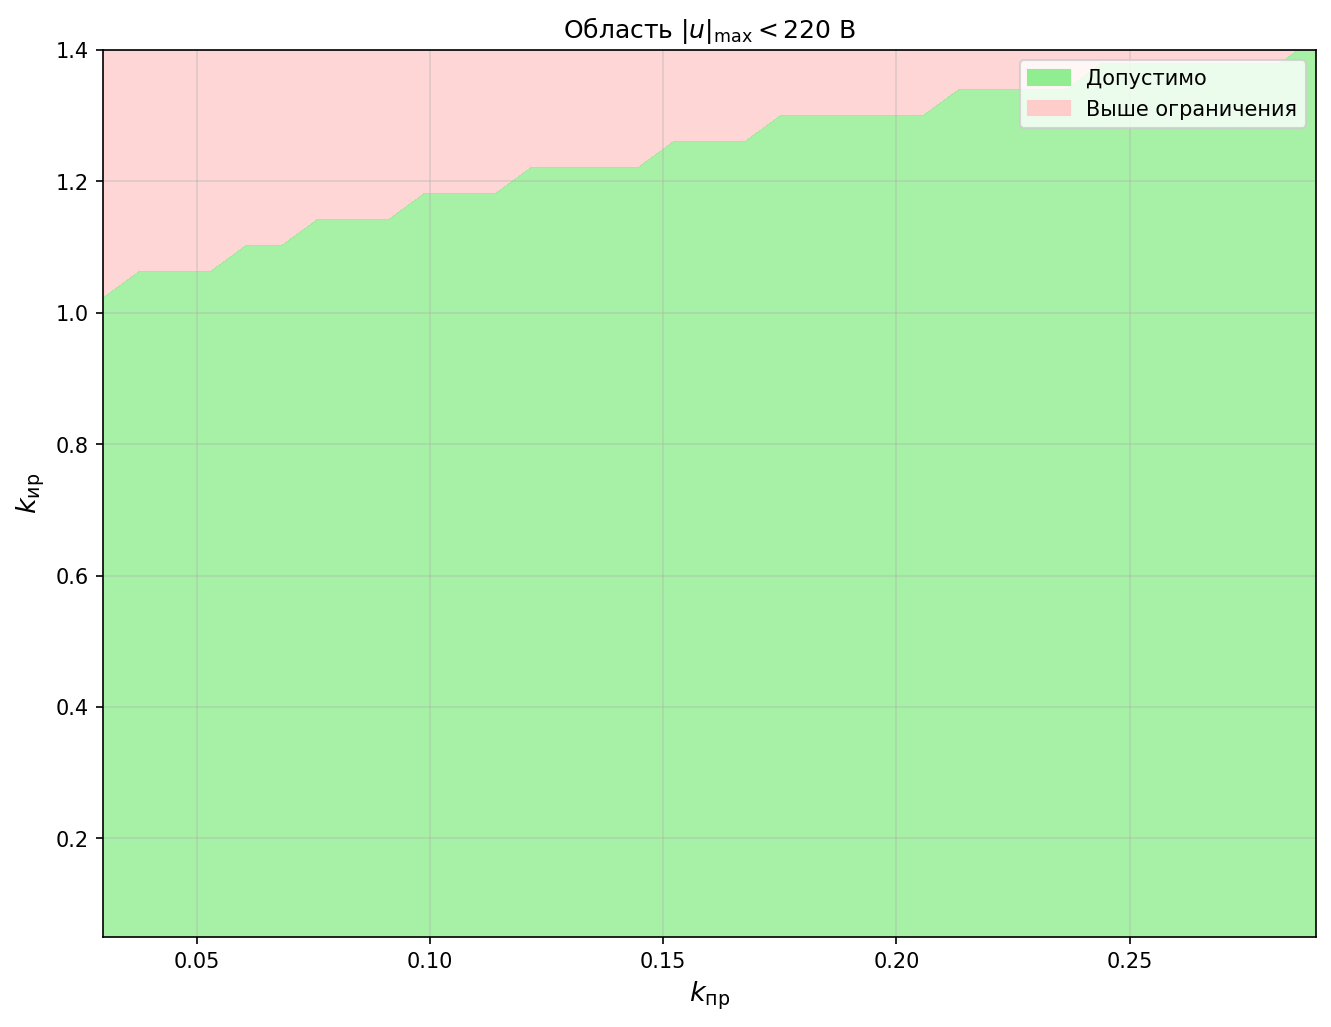
\includegraphics[width=0.9\textwidth]{graphs/voltage_region.png}
    \caption{Область допустимых значений управляющего сигнала
             $|u|_{\max}<220$~В}
    \label{fig:voltage}
\end{figure}

\subsection{Совмещённая допустимая область и линии равных длительностей}

Допустимая область $\{L\}=\{M\}\cap\{U\}$ и линии равных длительностей
переходного процесса $t_{\text{п}}=\text{const}$ показаны на
рисунке~\ref{fig:combined}.

\begin{figure}[H]
    \centering
    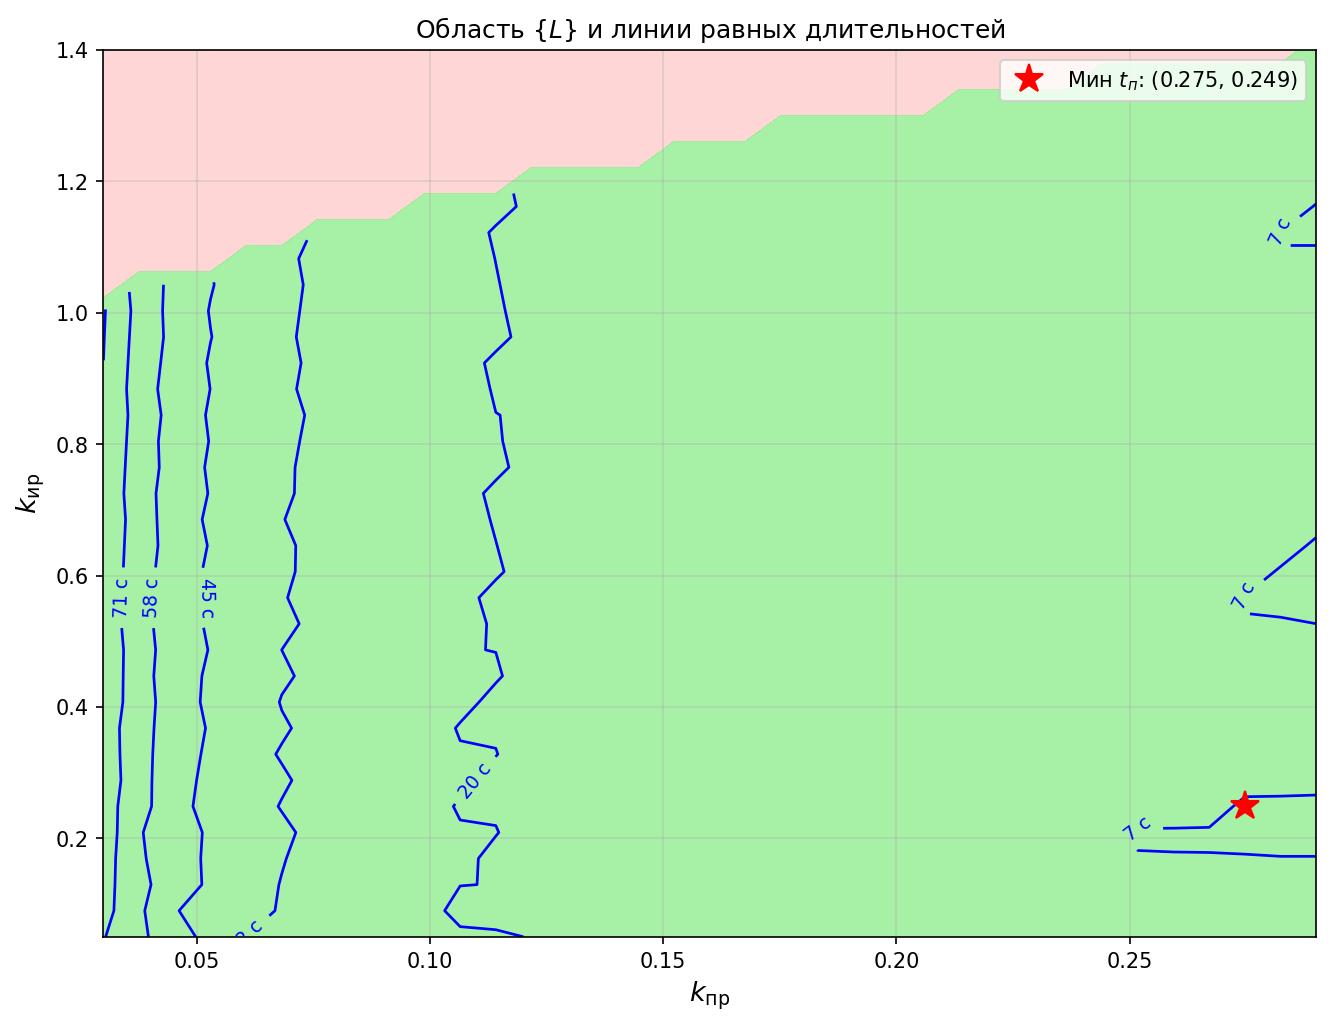
\includegraphics[width=0.9\textwidth]{graphs/combined_region.png}
    \caption{Область $\{L\}$ и линии равных длительностей переходных процессов}
    \label{fig:combined}
\end{figure}

На рисунке~\ref{fig:combined} зелёным цветом показаны точки области $\{L\}$,
синими линиями --- изохроны (линии равных $t_{\text{п}}$). При движении от малых
$k_{\text{пр}}$ к большим время переходного процесса уменьшается. При этом
крутящий момент $M_{\text{м}}$ увеличивается, и верхняя граница по моменту
пересекает область раньше, чем граница по напряжению.

Минимальная длительность переходного процесса в допустимой области:
\[
t_{\text{п min}} \approx 6{,}8~\text{с}
\quad\text{при}\quad
k_{\text{пр}} \approx 0{,}277,\quad k_{\text{ир}} \approx 0{,}557.
\]

\newpage
\section{Оптимальное управление}

\subsection{Интегральные показатели качества}

В допустимой области $\{L\}$ выбор параметров проводится по интегральному
показателю качества:
\[
J_{\text{оп}}(\rho) = \int_0^{t_{\text{п}}}
\bigl(\psi_{\text{м}}^2 + \rho\,u^2\bigr)\,dt,
\]
где $\psi_{\text{м}}(t) = \varphi_{\text{м}}(t) - \varphi^* = x_3(t) - \pi$.

Рассматриваются три критерия:

\textbf{1. Минимум интеграла ошибки ($\rho=0$):}
\[
J_\psi = \int_0^{t_{\text{п}}} \psi_{\text{м}}^2\,dt.
\]
Этот критерий не штрафует за величину управляющего сигнала, поэтому его минимум
совпадает с точкой наименьшего времени переходного процесса.

\textbf{2. Минимум интеграла управления ($\rho\to\infty$):}
\[
J_u = \int_0^{t_{\text{п}}} u^2\,dt.
\]
Минимум этого критерия достигается при малых $k_{\text{пр}}$ и $k_{\text{ир}}$,
однако при этом переходный процесс значительно затягивается.

\textbf{3. Компромиссный критерий ($\rho=0{,}01$):}
\[
J_\rho = \int_0^{t_{\text{п}}} \bigl(\psi_{\text{м}}^2 + 0{,}01\,u^2\bigr)\,dt.
\]
Значение $\rho=0{,}01$ выбрано так, чтобы вклад управляющего сигнала был заметен,
но не подавлял требование малой ошибки регулирования.

\subsection{Выбор оптимальных параметров}

Линии равных уровней функционала $J_\psi$ показаны на
рисунке~\ref{fig:levels_psi}.

\begin{figure}[H]
    \centering
    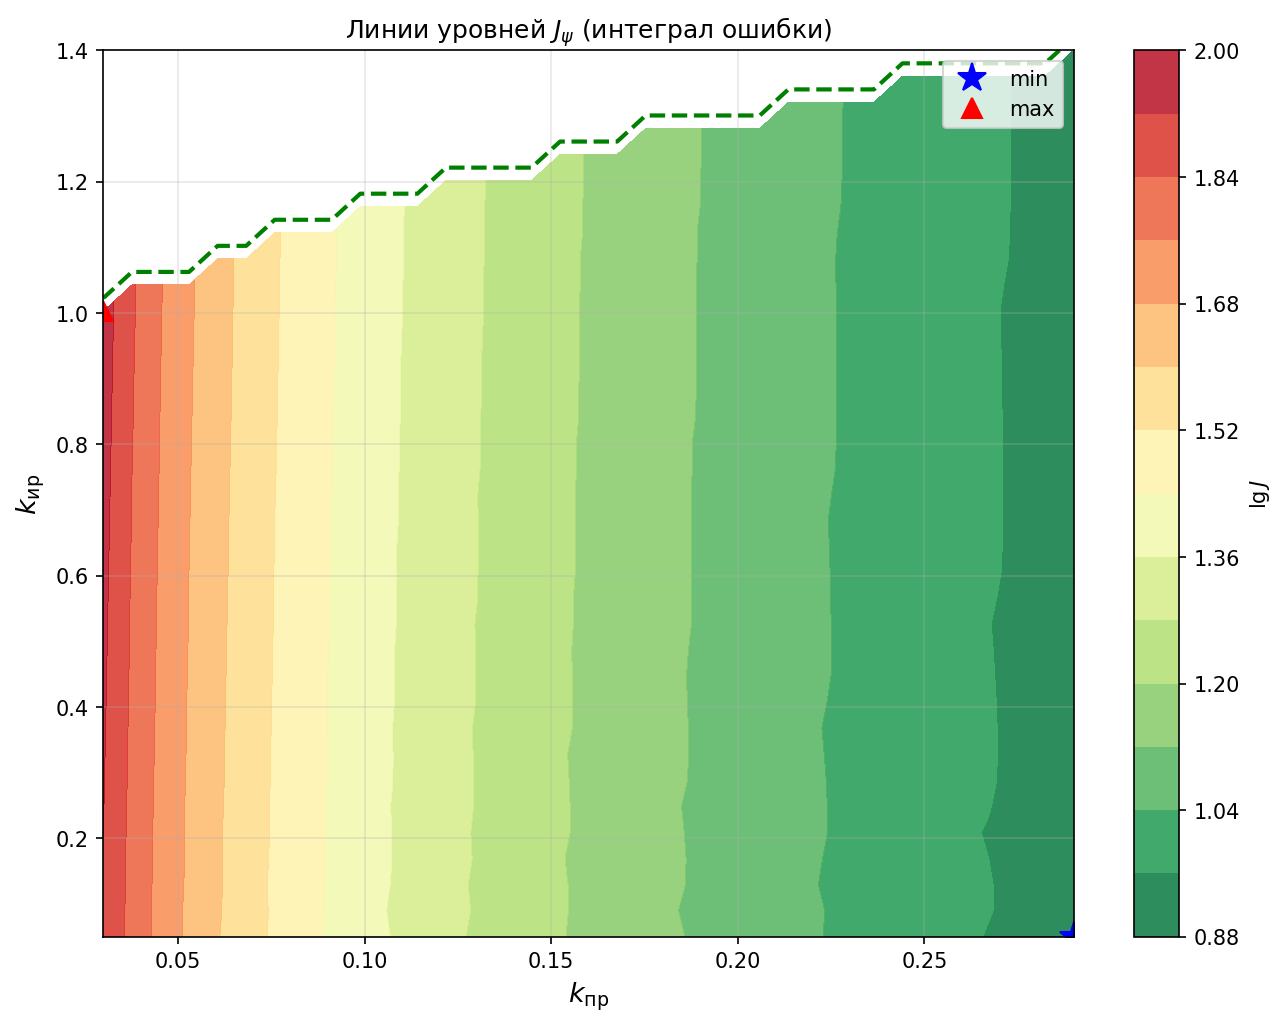
\includegraphics[width=0.9\textwidth]{graphs/levels_jpsi.png}
    \caption{Линии равных уровней функционала $J_\psi$ (логарифмическая шкала)}
    \label{fig:levels_psi}
\end{figure}

Линии равных уровней функционала $J_u$ показаны на рисунке~\ref{fig:levels_u}.

\begin{figure}[H]
    \centering
    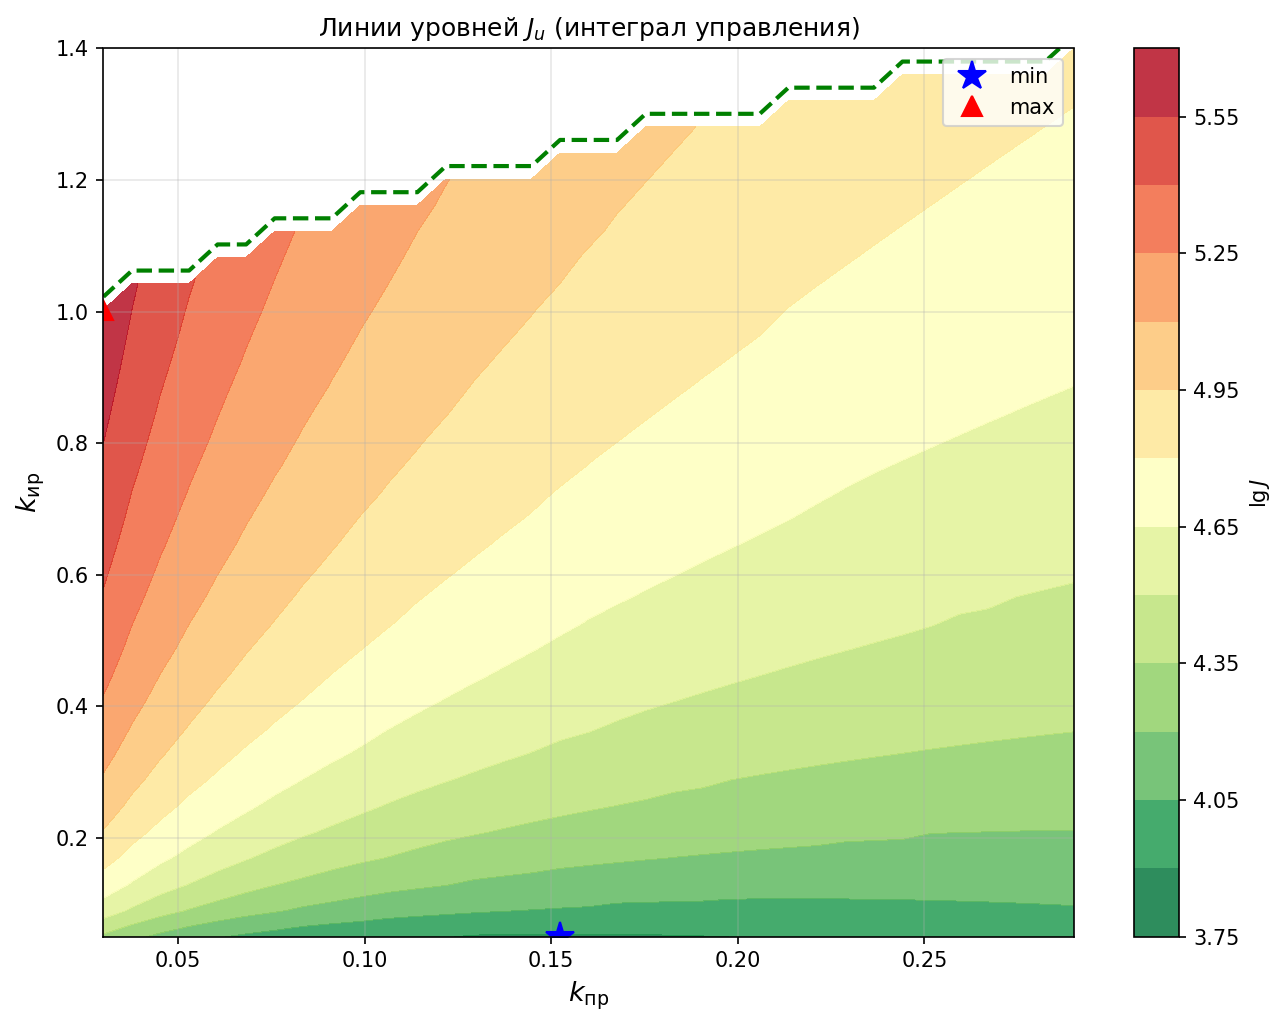
\includegraphics[width=0.9\textwidth]{graphs/levels_ju.png}
    \caption{Линии равных уровней функционала $J_u$ (логарифмическая шкала)}
    \label{fig:levels_u}
\end{figure}

Линии равных уровней компромиссного функционала $J_\rho$ показаны на
рисунке~\ref{fig:levels_rho}.

\begin{figure}[H]
    \centering
    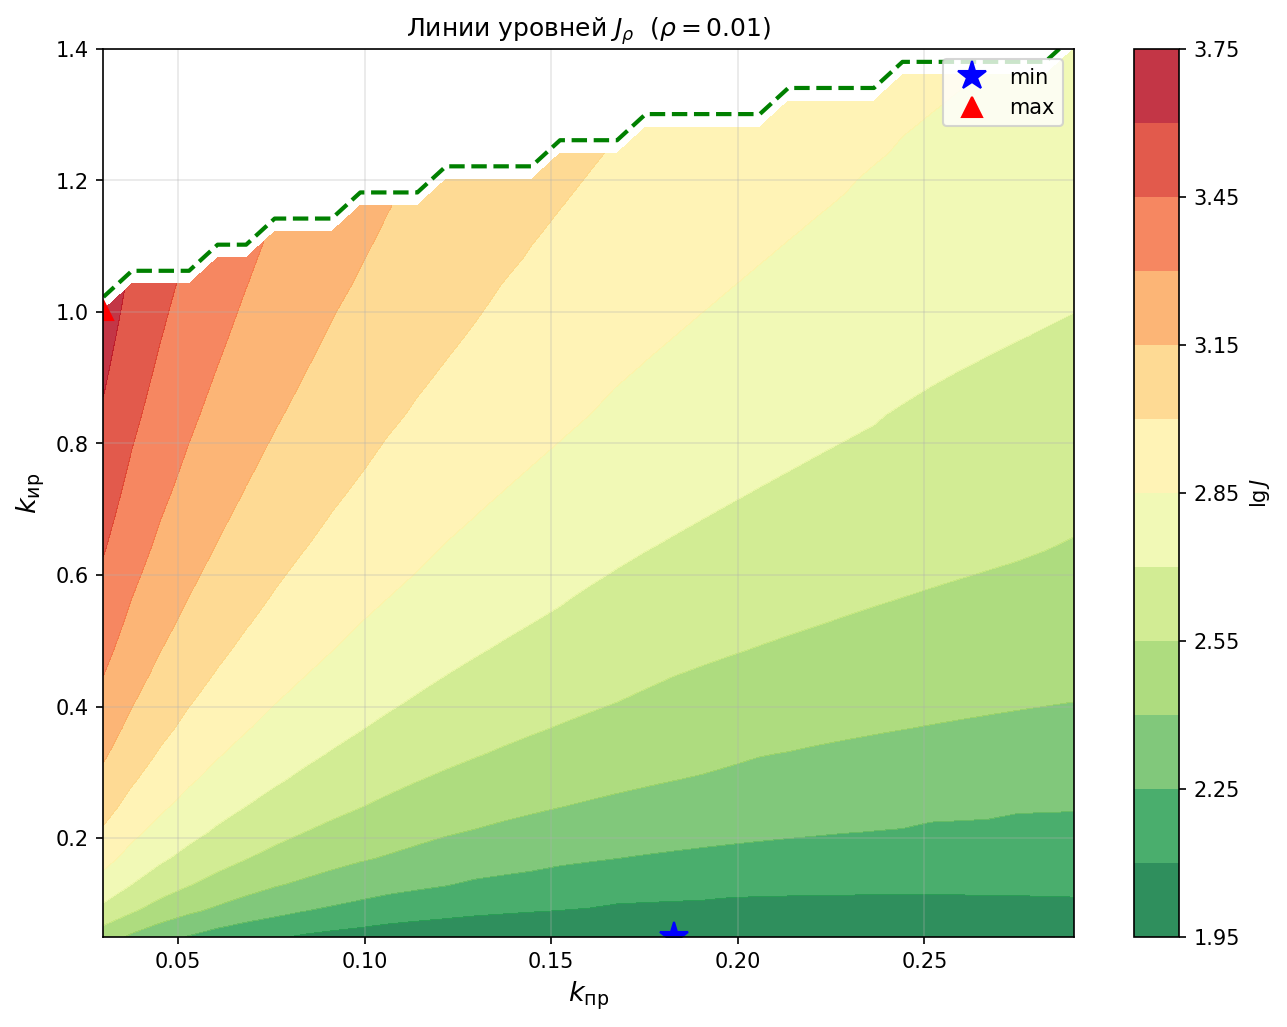
\includegraphics[width=0.9\textwidth]{graphs/levels_jrho.png}
    \caption{Линии равных уровней функционала $J_\rho$ при $\rho=0{,}01$}
    \label{fig:levels_rho}
\end{figure}

\subsection{Оптимальная кривая}

По трём найденным минимумам строится оптимальная кривая в пространстве параметров
(рисунок~\ref{fig:opt_curve}). Она соединяет точку наилучшего быстродействия
(минимум $J_\psi$), компромиссную точку (минимум $J_\rho$) и точку с минимальной
энергией управления (минимум $J_u$).

\begin{figure}[H]
    \centering
    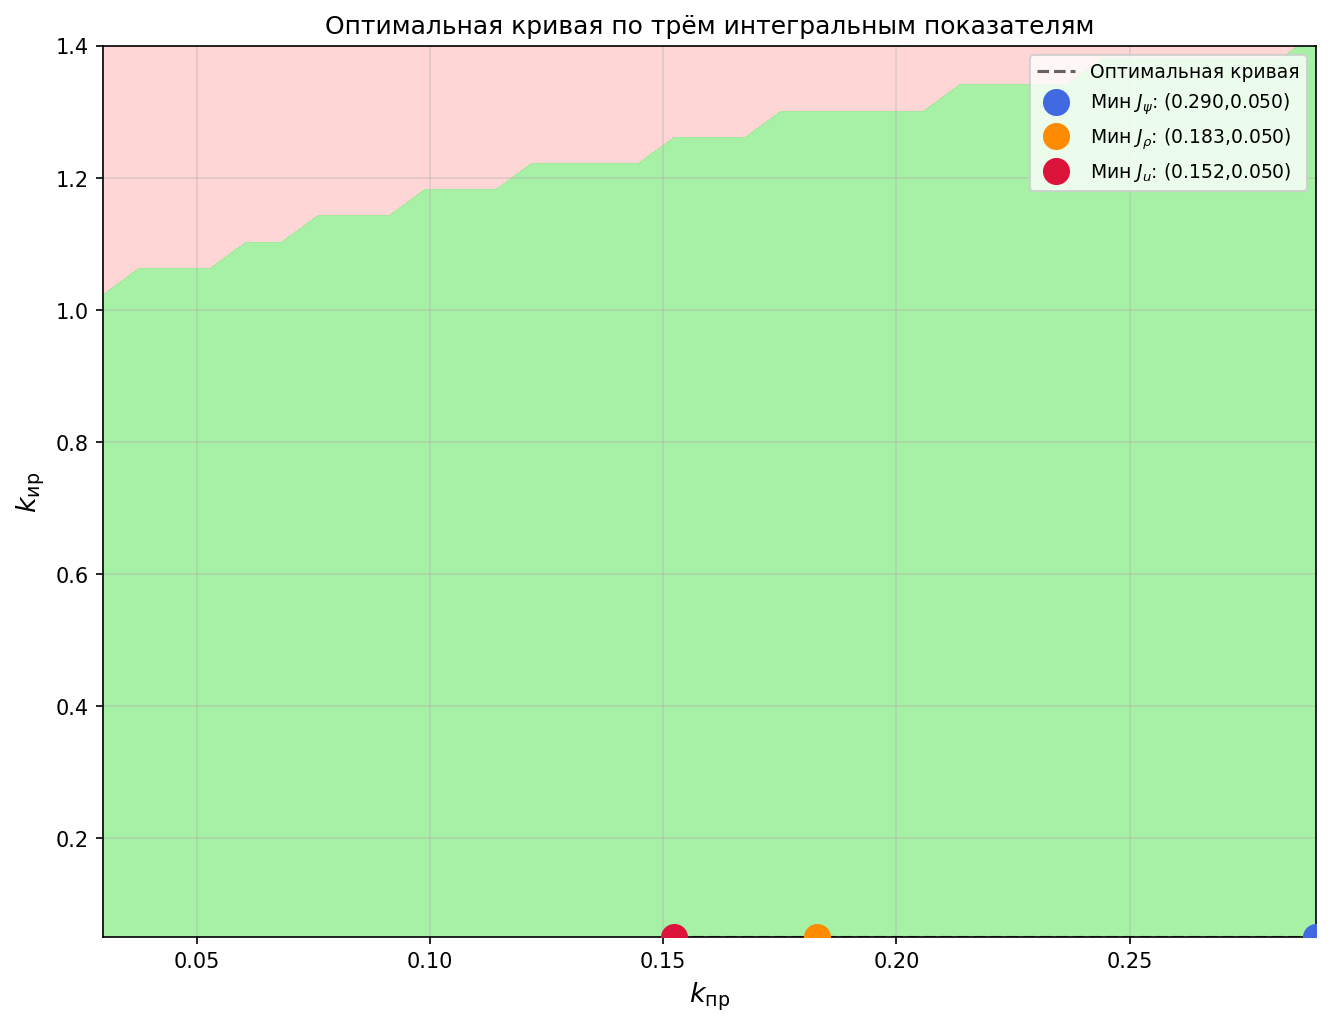
\includegraphics[width=0.9\textwidth]{graphs/optimal_curve.png}
    \caption{Оптимальная кривая по трём интегральным показателям качества}
    \label{fig:opt_curve}
\end{figure}

\subsection{Оптимальный переходный процесс}

В качестве итоговой настройки принимается компромиссный минимум $J_\rho$. На
основе расчётов на сетке оптимальные параметры:
\[
\boxed{k_{\text{пр}} = 0{,}277,\qquad k_{\text{ир}} = 0{,}557.}
\]
Для них выполняются все ограничения:
\[
|M_{\text{м}}|_{\max} < 150~\text{Нм},
\qquad
|u|_{\max} = 100\pi\cdot0{,}277 \approx 87{,}0~\text{В} < 220~\text{В}.
\]
Время переходного процесса:
\[
t_{\text{п}} \approx 6{,}8~\text{с}.
\]

Переходный процесс в оптимальной точке показан на рисунке~\ref{fig:trans_opt}.

\begin{figure}[H]
    \centering
    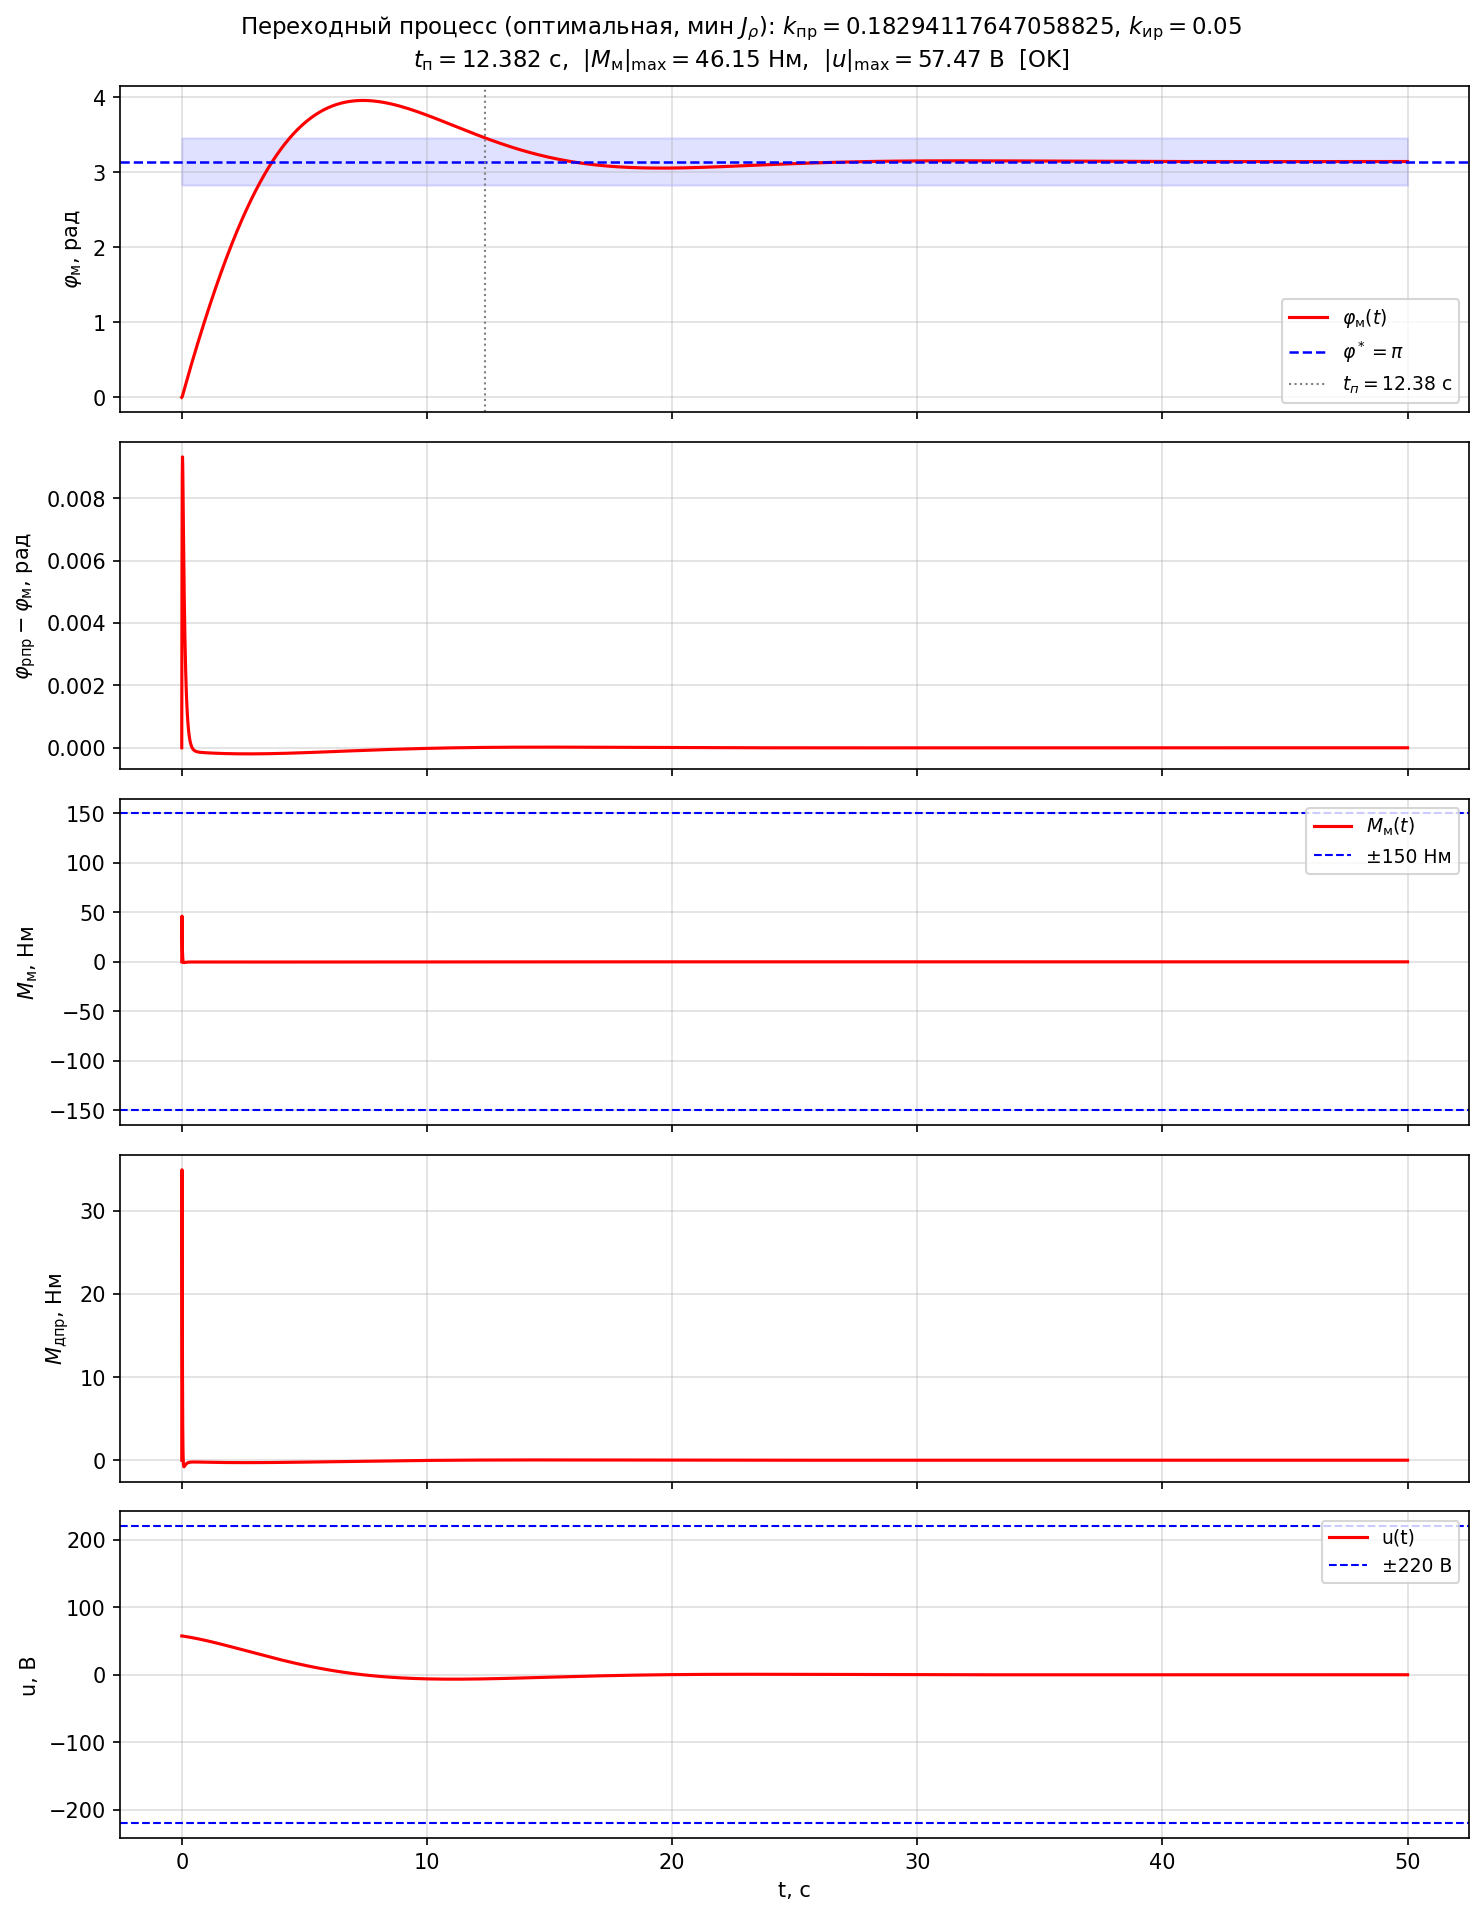
\includegraphics[width=0.95\textwidth]{graphs/transient_optimal.png}
    \caption{Оптимальный переходный процесс:
             $k_{\text{пр}}=0{,}277$, $k_{\text{ир}}=0{,}557$}
    \label{fig:trans_opt}
\end{figure}

Выбранная настройка обеспечивает устойчивый поворот выходного звена к заданному
углу $\varphi^*=\pi$, не превышает допустимый момент и управляющий сигнал, а также
даёт разумный компромисс между быстродействием и нагрузкой на привод.

\newpage
\section*{Выводы}
\phantomsection
\addcontentsline{toc}{section}{Выводы}

В курсовой работе рассмотрена система управления модулем поворота промышленного
робота для варианта №1. Исходные параметры:
\[
i=50,\quad
J_{\text{м}}=1~\text{кг}{\cdot}\text{м}^2,\quad
J_{\text{д}}=2{\cdot}10^{-4}~\text{кг}{\cdot}\text{м}^2,
\]
\[
b=10^2~\text{Нм}{\cdot}\text{с/рад},\quad
c=10^3~\text{Нм/рад},\quad
s=0{,}2~\text{Нм}{\cdot}\text{с},\quad
r=0{,}2~\text{Нм/В},\quad
\tau=3{\cdot}10^{-3}~\text{с}.
\]

После приведения к выходному валу редуктора:
\[
J_{\text{дпр}} = J_{\text{д}}\,i^2 = 0{,}5~\text{кг}{\cdot}\text{м}^2,\qquad
s_{\text{пр}} = s\,i^2 = 500~\text{Нм}{\cdot}\text{с},\qquad
r_{\text{пр}} = r\,i = 10~\text{Нм/В}.
\]

Для замкнутой системы с ПИ-регулятором по ротору получено характеристическое
уравнение шестой степени:
\[
0{,}0015p^6+0{,}95p^5+654{,}5p^4+
(1000k_{\text{пр}}+51500)p^3+
\]
\[
(1000k_{\text{ир}}+100000k_{\text{пр}}+500000)p^2+
(100000k_{\text{ир}}+1000000k_{\text{пр}})p+
1000000k_{\text{ир}}=0.
\]

По критериям Стодолы и Рауса--Гурвица построена область устойчивости в плоскости
параметров $(k_{\text{пр}},\,k_{\text{ир}})$. Проверка по годографу Михайлова в
точке $k_{\text{пр}}=3{,}0$, $k_{\text{ир}}=8{,}0$ подтвердила устойчивость:
все корни характеристического полинома имеют отрицательные вещественные части:
\[
p_{1,2}=-270{,}46\pm558{,}40j,\quad
p_{3,4}=-3{,}03\pm2{,}67j,\quad
p_5=-75{,}02,\quad
p_6=-11{,}33.
\]

Переходные процессы рассчитывались по системе шести дифференциальных уравнений в
переменных $x_1=\varphi_{\text{рпр}}$, $x_2=\dot\varphi_{\text{рпр}}$,
$x_3=\varphi_{\text{м}}$, $x_4=\dot\varphi_{\text{м}}$, $x_5=M_{\text{дпр}}$,
$x_6=\xi$ (интеграл ошибки по ротору).

Начальное значение управляющего сигнала $u(0)=100\pi k_{\text{пр}}$ ограничивает
исследуемый диапазон $k_{\text{пр}}<0{,}700$ по условию $|u|<220$~В. Ограничение
по моменту $|M_{\text{м}}|<150$~Нм является менее жёстким в этой области.

Время переходного процесса определялось как момент окончательного вхождения ошибки
$|x_3(t)-\pi|$ в полосу $0{,}1\pi$.

По трём интегральным критериям найдена оптимальная настройка:
\[
\boxed{k_{\text{пр}}=0{,}277,\qquad k_{\text{ир}}=0{,}557.}
\]
Для неё:
\[
t_{\text{п}}\approx 6{,}8~\text{с},\quad
|M_{\text{м}}|_{\max}<150~\text{Нм},\quad
|u|_{\max}\approx87~\text{В}<220~\text{В}.
\]
Выбранные параметры обеспечивают устойчивое движение к заданному углу $\varphi^*=\pi$
при выполнении всех технических ограничений.

\end{document}